\documentclass{article}

\usepackage[margin=1in]{geometry}
\usepackage{amsmath,amssymb}
\usepackage{graphicx}

\renewcommand{\thesection}{Exercise \arabic{section}}

\begin{document}

\title{ex. session 1 IMS}
\author{By George Viorel Visniuc}
\maketitle



\section{}


\begin{gather}
\text{a) To calculate the intensity for I and S we use the formula}\ \frac{R + G + B}{3} \text{ in our case }\ \frac{X + Y + Z}{3} \\
I_{S} = \frac{300}{3} = 100 \\
I_{A} = \frac{350}{3} = 116,1
\end{gather}

b) The chromaticity values are :
\begin{gather}  
x_{S} = \frac{100}{300} = \frac{1}{3} \\
y_{S} = \frac{100}{300} = \frac{1}{3} \\
x_{A} = \frac{100}{350} = 0.28 \\
y_{A} = \frac{100}{350} = 0.28 \\
\end{gather}
\begin{center}
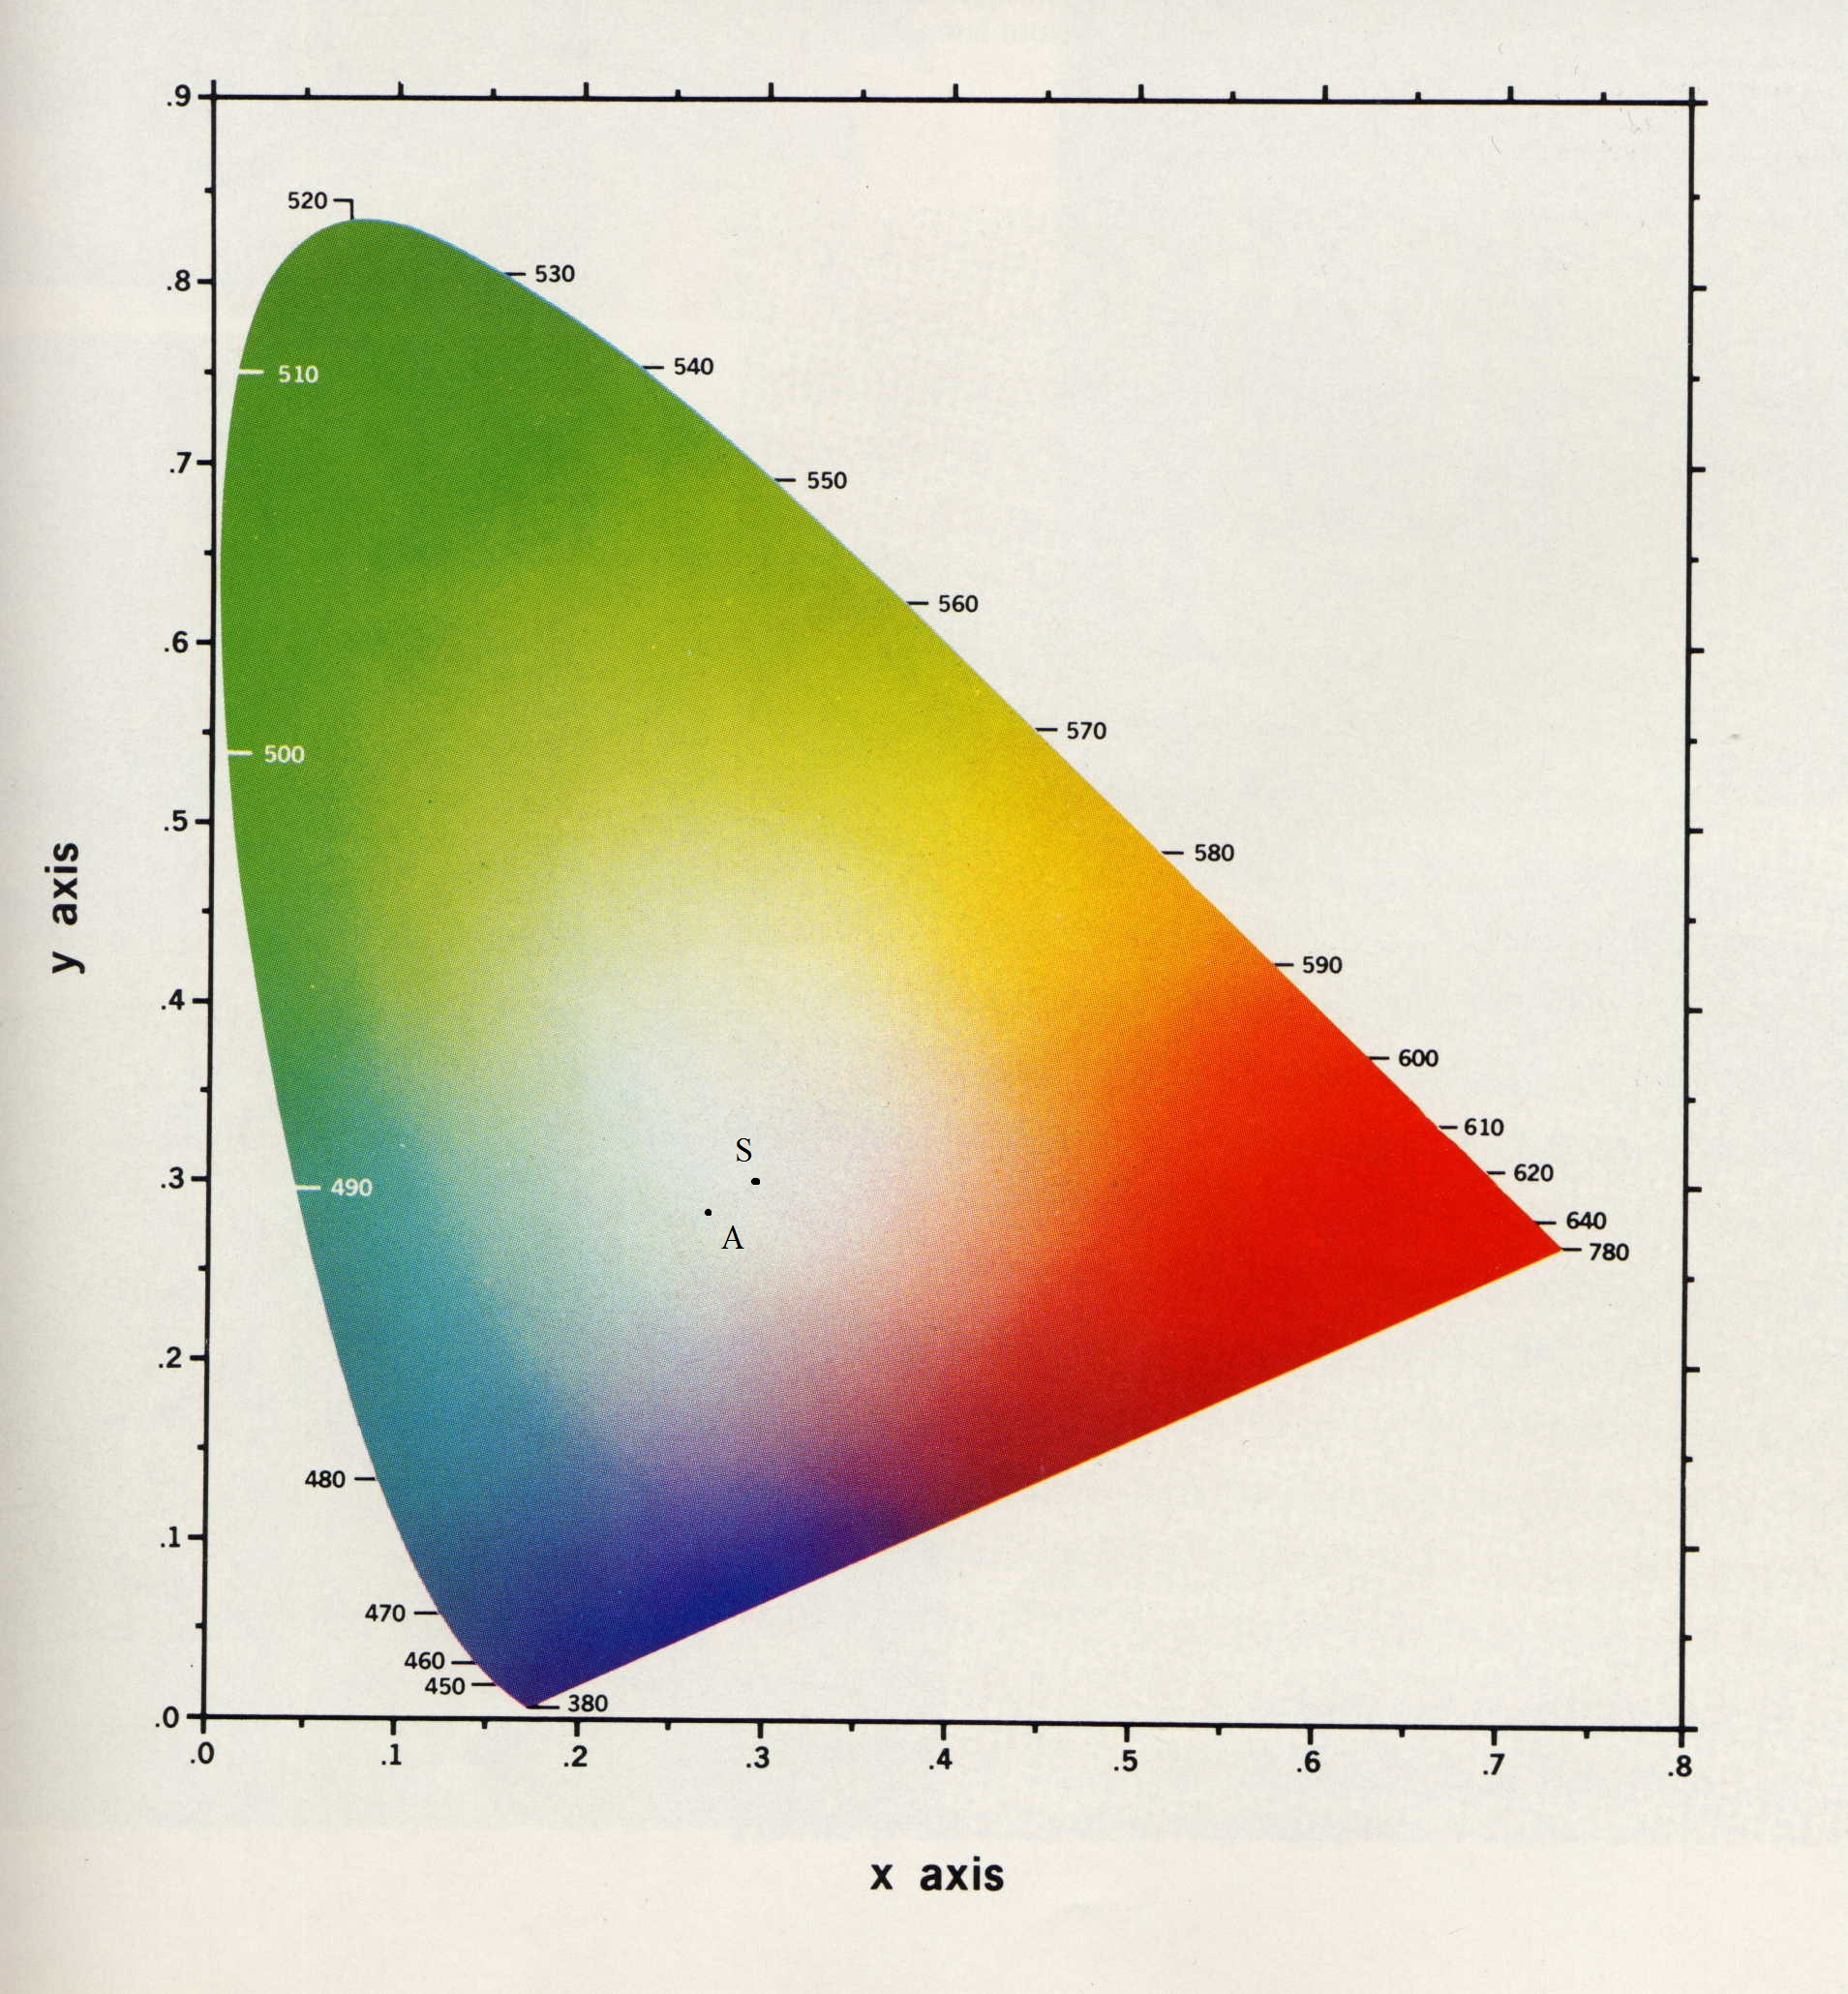
\includegraphics[width=0.4\textwidth]{b1.jpg} 
\end{center}
c)Hue is:
\begin{gather}  
\text{ Having already calculated the chromaticity values for A and S }\ \\
x_{B} = \frac{x_{B}}{x_{B}+y_{B}+z_{B}} = \frac{120}{320} = 0.375 \\
y_{B} = \frac{y_{B}}{x_{B}+y_{B}+z_{B}} = \frac{100}{350} = 0.31 \\
\end{gather}
\begin{center}
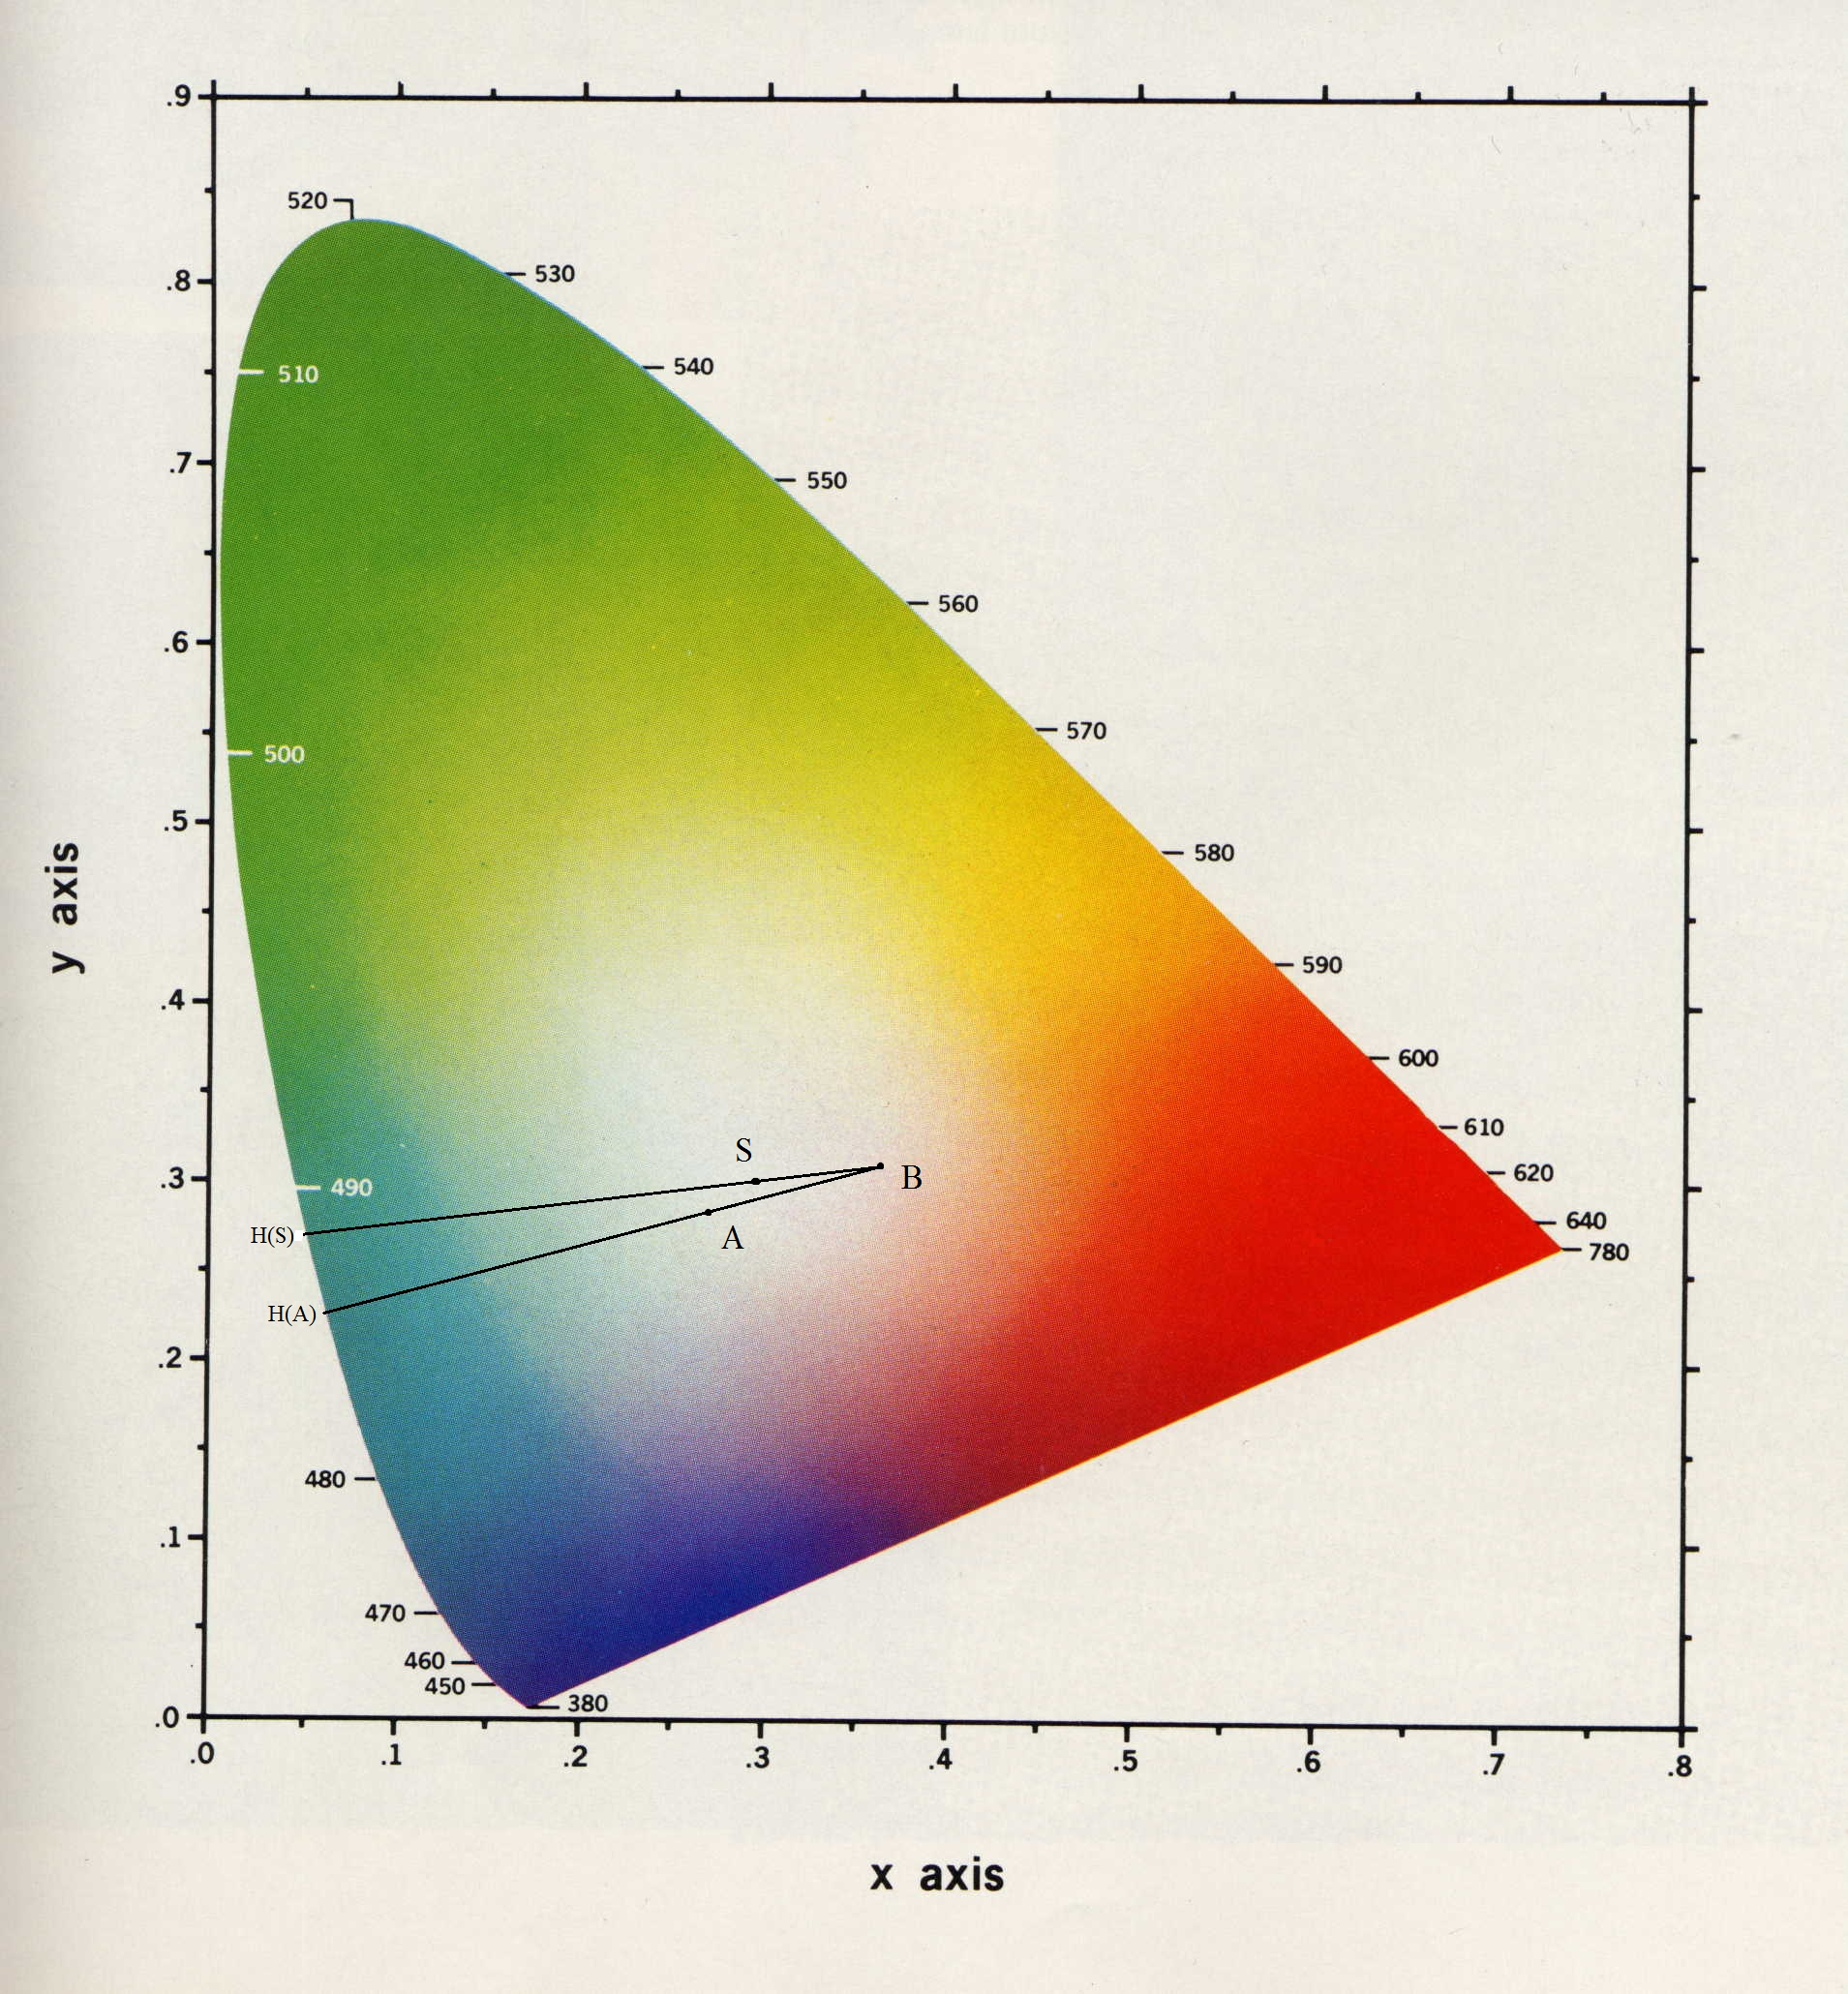
\includegraphics[width=0.4\textwidth]{c.jpg} 
\end{center}
d)Saturation is higher when the values are closer to the edge. In our case :
\begin{gather}  
S_{A} > S_{B}
\end{gather}
e) The region of colors is:
\begin{center}
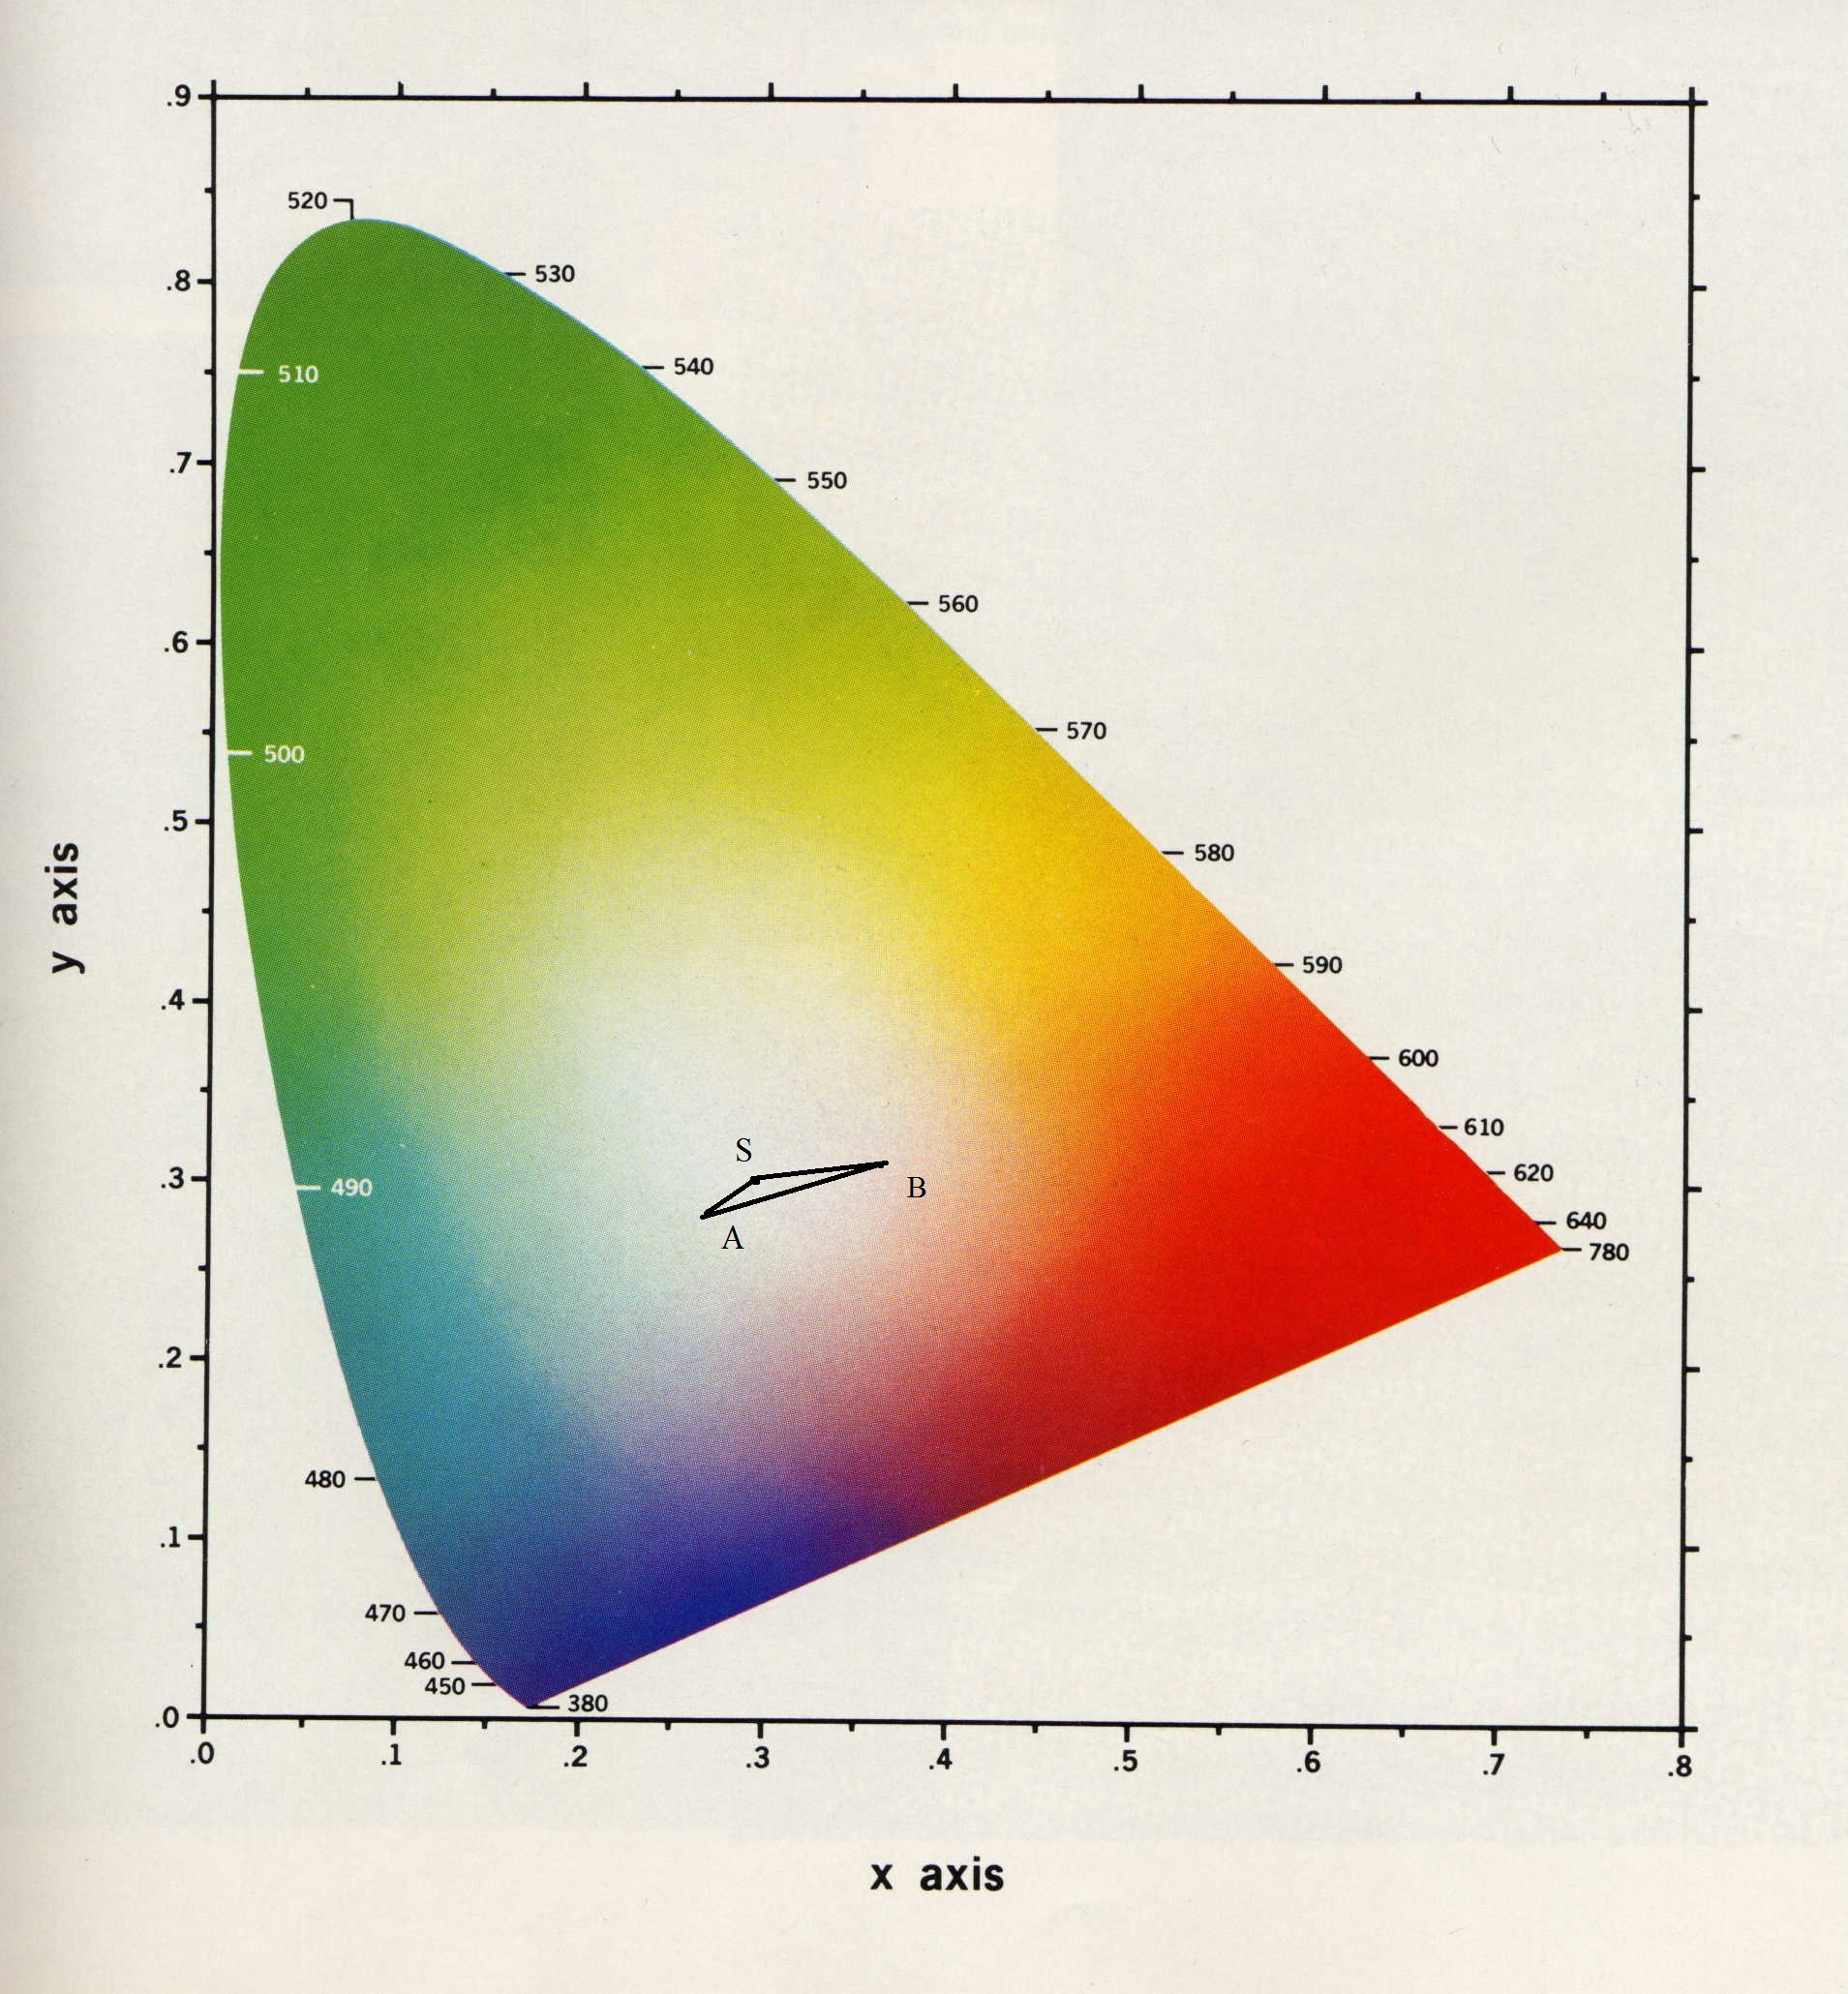
\includegraphics[width=0.4\textwidth]{e.jpg} 
\end{center}
\section{}
a) X, Y and Z are:
\begin{gather}  
X = \int_\lambda k(\lambda) \bar{x}(\lambda) d{\lambda} \text{  }\ | \text{  }\ k({\lambda}) = k\\ 
X = k \int_\lambda \bar{x}(\lambda) d{\lambda} \text{  }\ | \text{  }\ {\lambda} = 500nm\\
X = k \int_\lambda \rho(\lambda) \bar{x}(\lambda) d{\lambda} \text{  }\ | \text{  }\ \rho(\lambda) = \rho(\lambda_{500})  \\ 
X = k \rho(\lambda_{500}) \bar{x}(\lambda_{500}) \\
X = k \bar{x}(\lambda_{500}) = k 0.0049 \\
\text{we repeat for y and z}\ \\
Y = k \bar{y}(\lambda_{500}) = k 0.323 \\
Y = k \bar{z}(\lambda_{500}) = k 0.272\\ 
\end{gather}
The chromaticity coordinates are :
\begin{gather}  
x_{A} = \frac{X_{A}}{X_{A}+Y_{A}+Z_{A}} = \frac{0.0049}{0.0049+0.323+0.272} = 0.0081 \\
y_{A} = 0.538 \\
z_{A} = 0.453 \\
\end{gather}
b)
\begin{center}
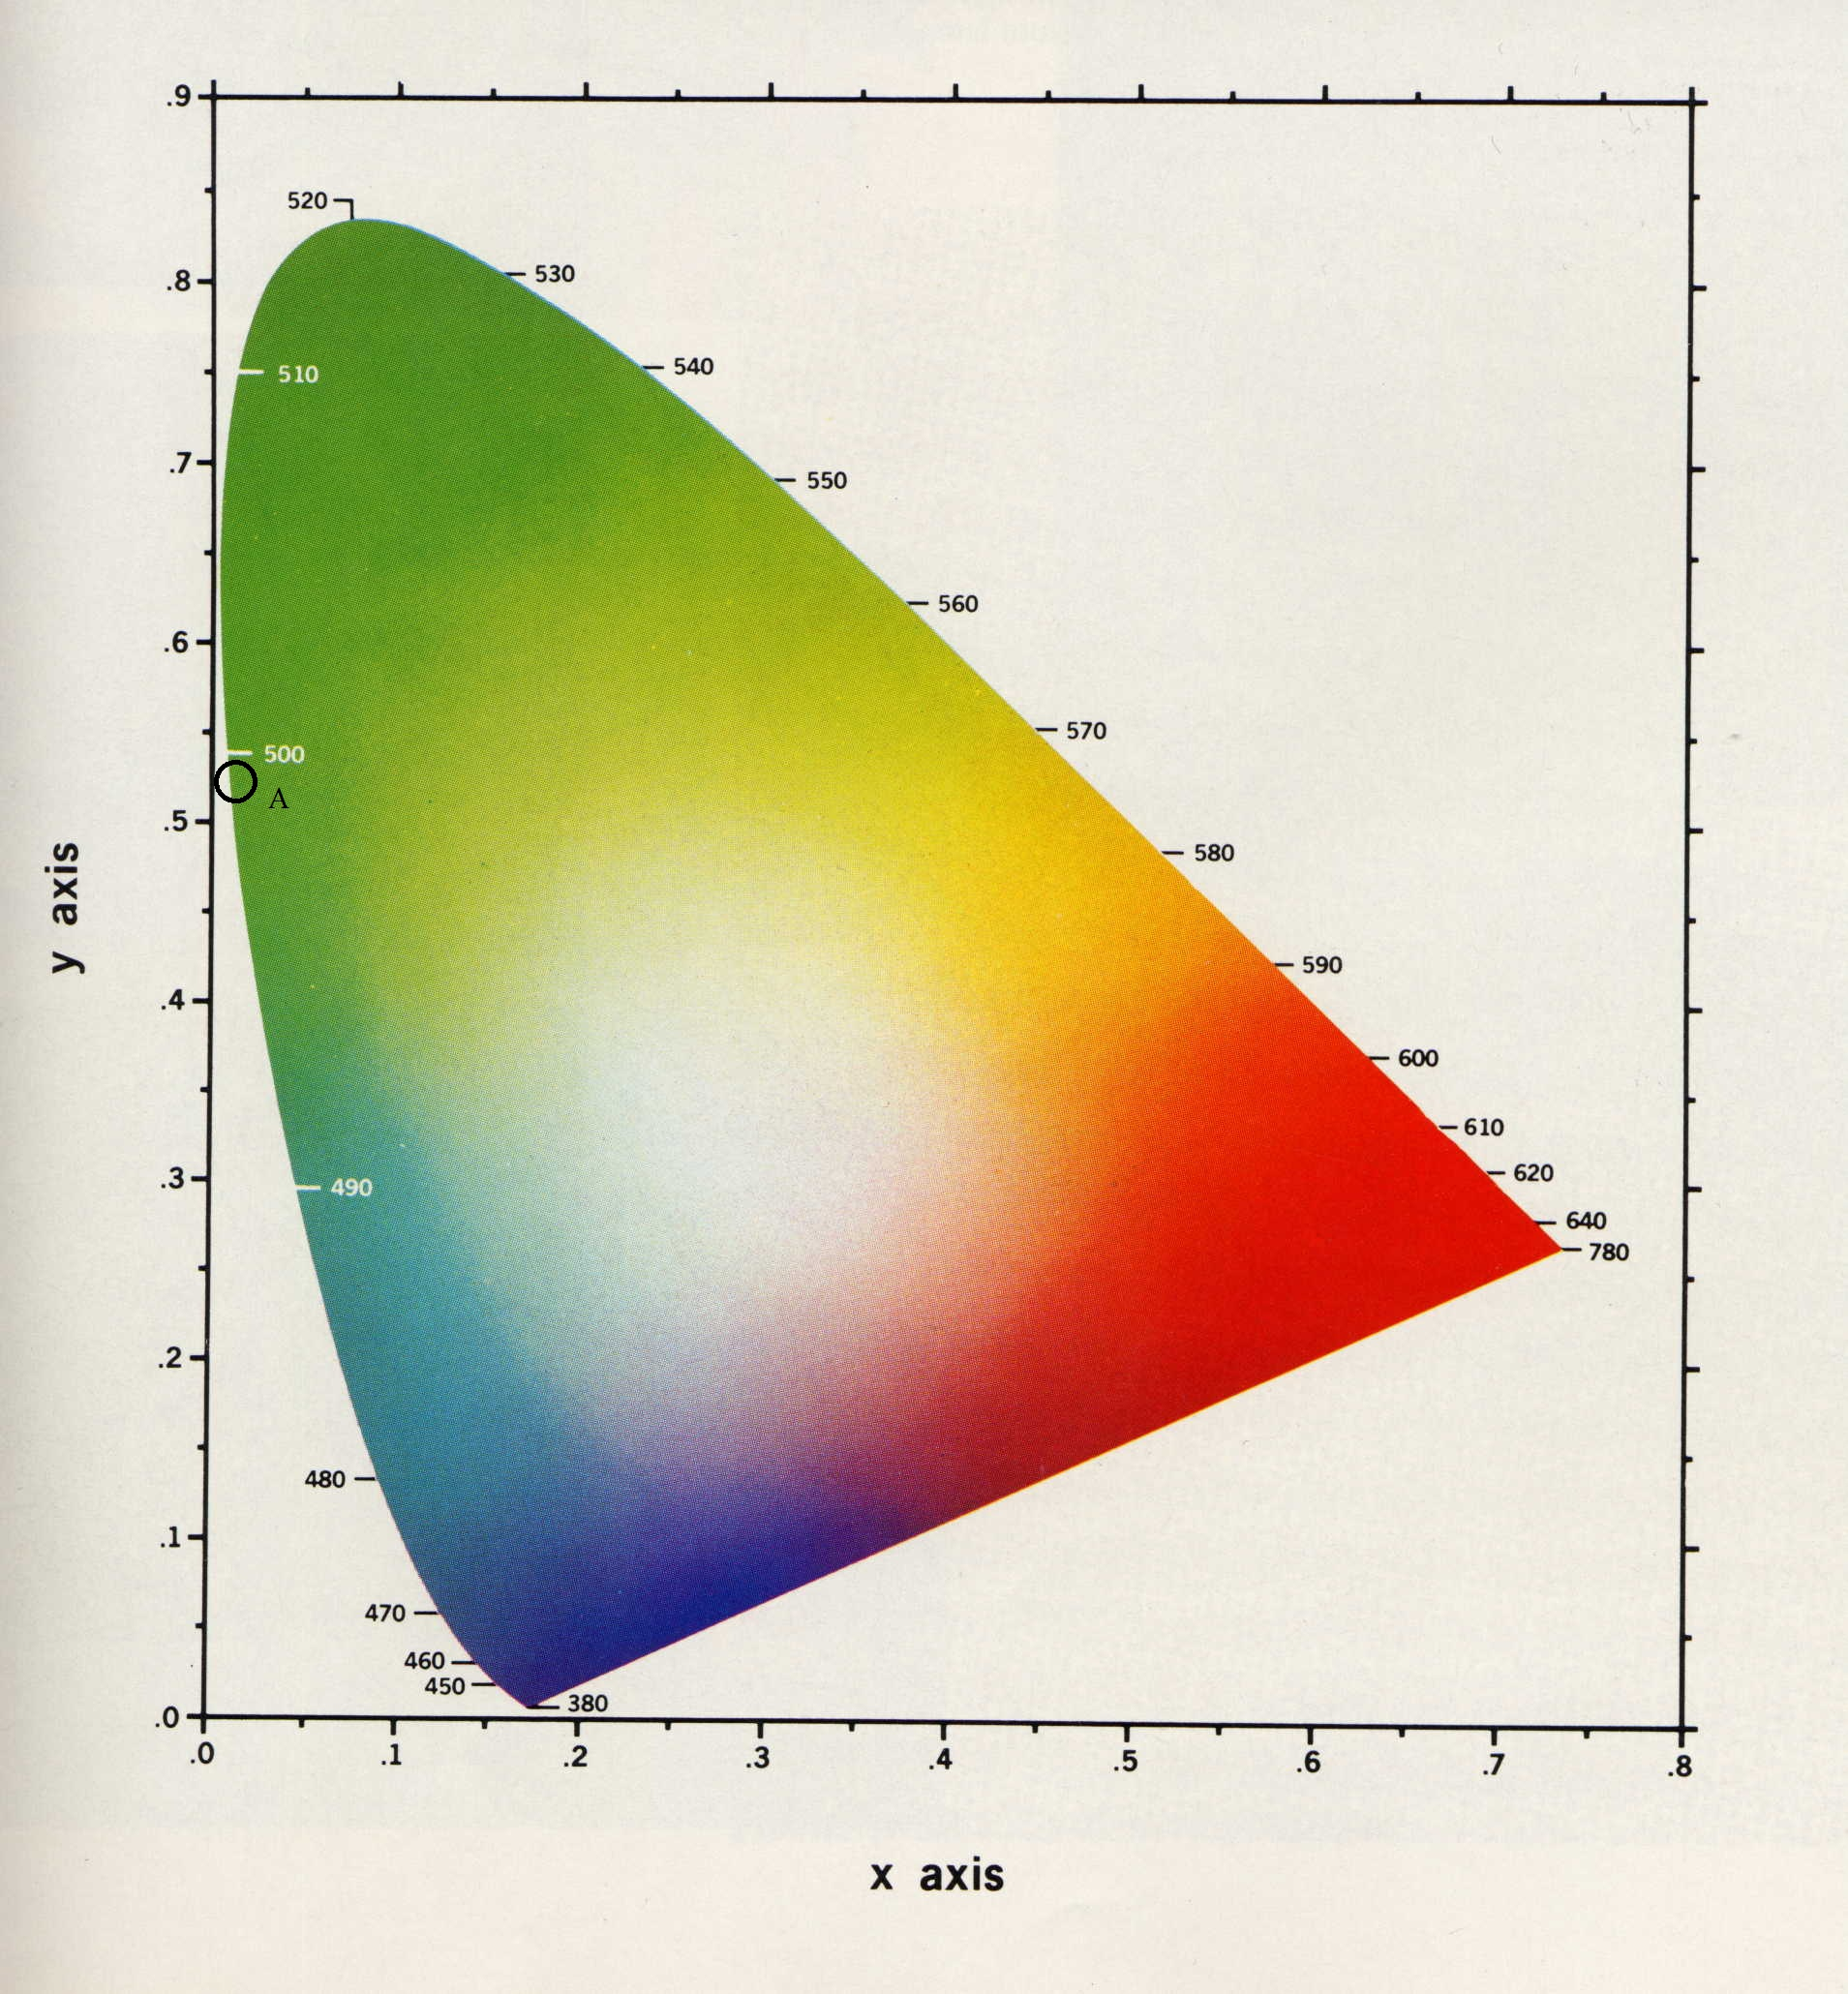
\includegraphics[width=0.4\textwidth]{2b.jpg} 
\end{center}
c) We repeat the process described in a). The chromaticity coordinates are :
\begin{gather} 
x_{B} = 0.51 \\
y_{B} = 0.48 \\
z_{B} = 0.0009 \\
\end{gather}
d)
\begin{center}
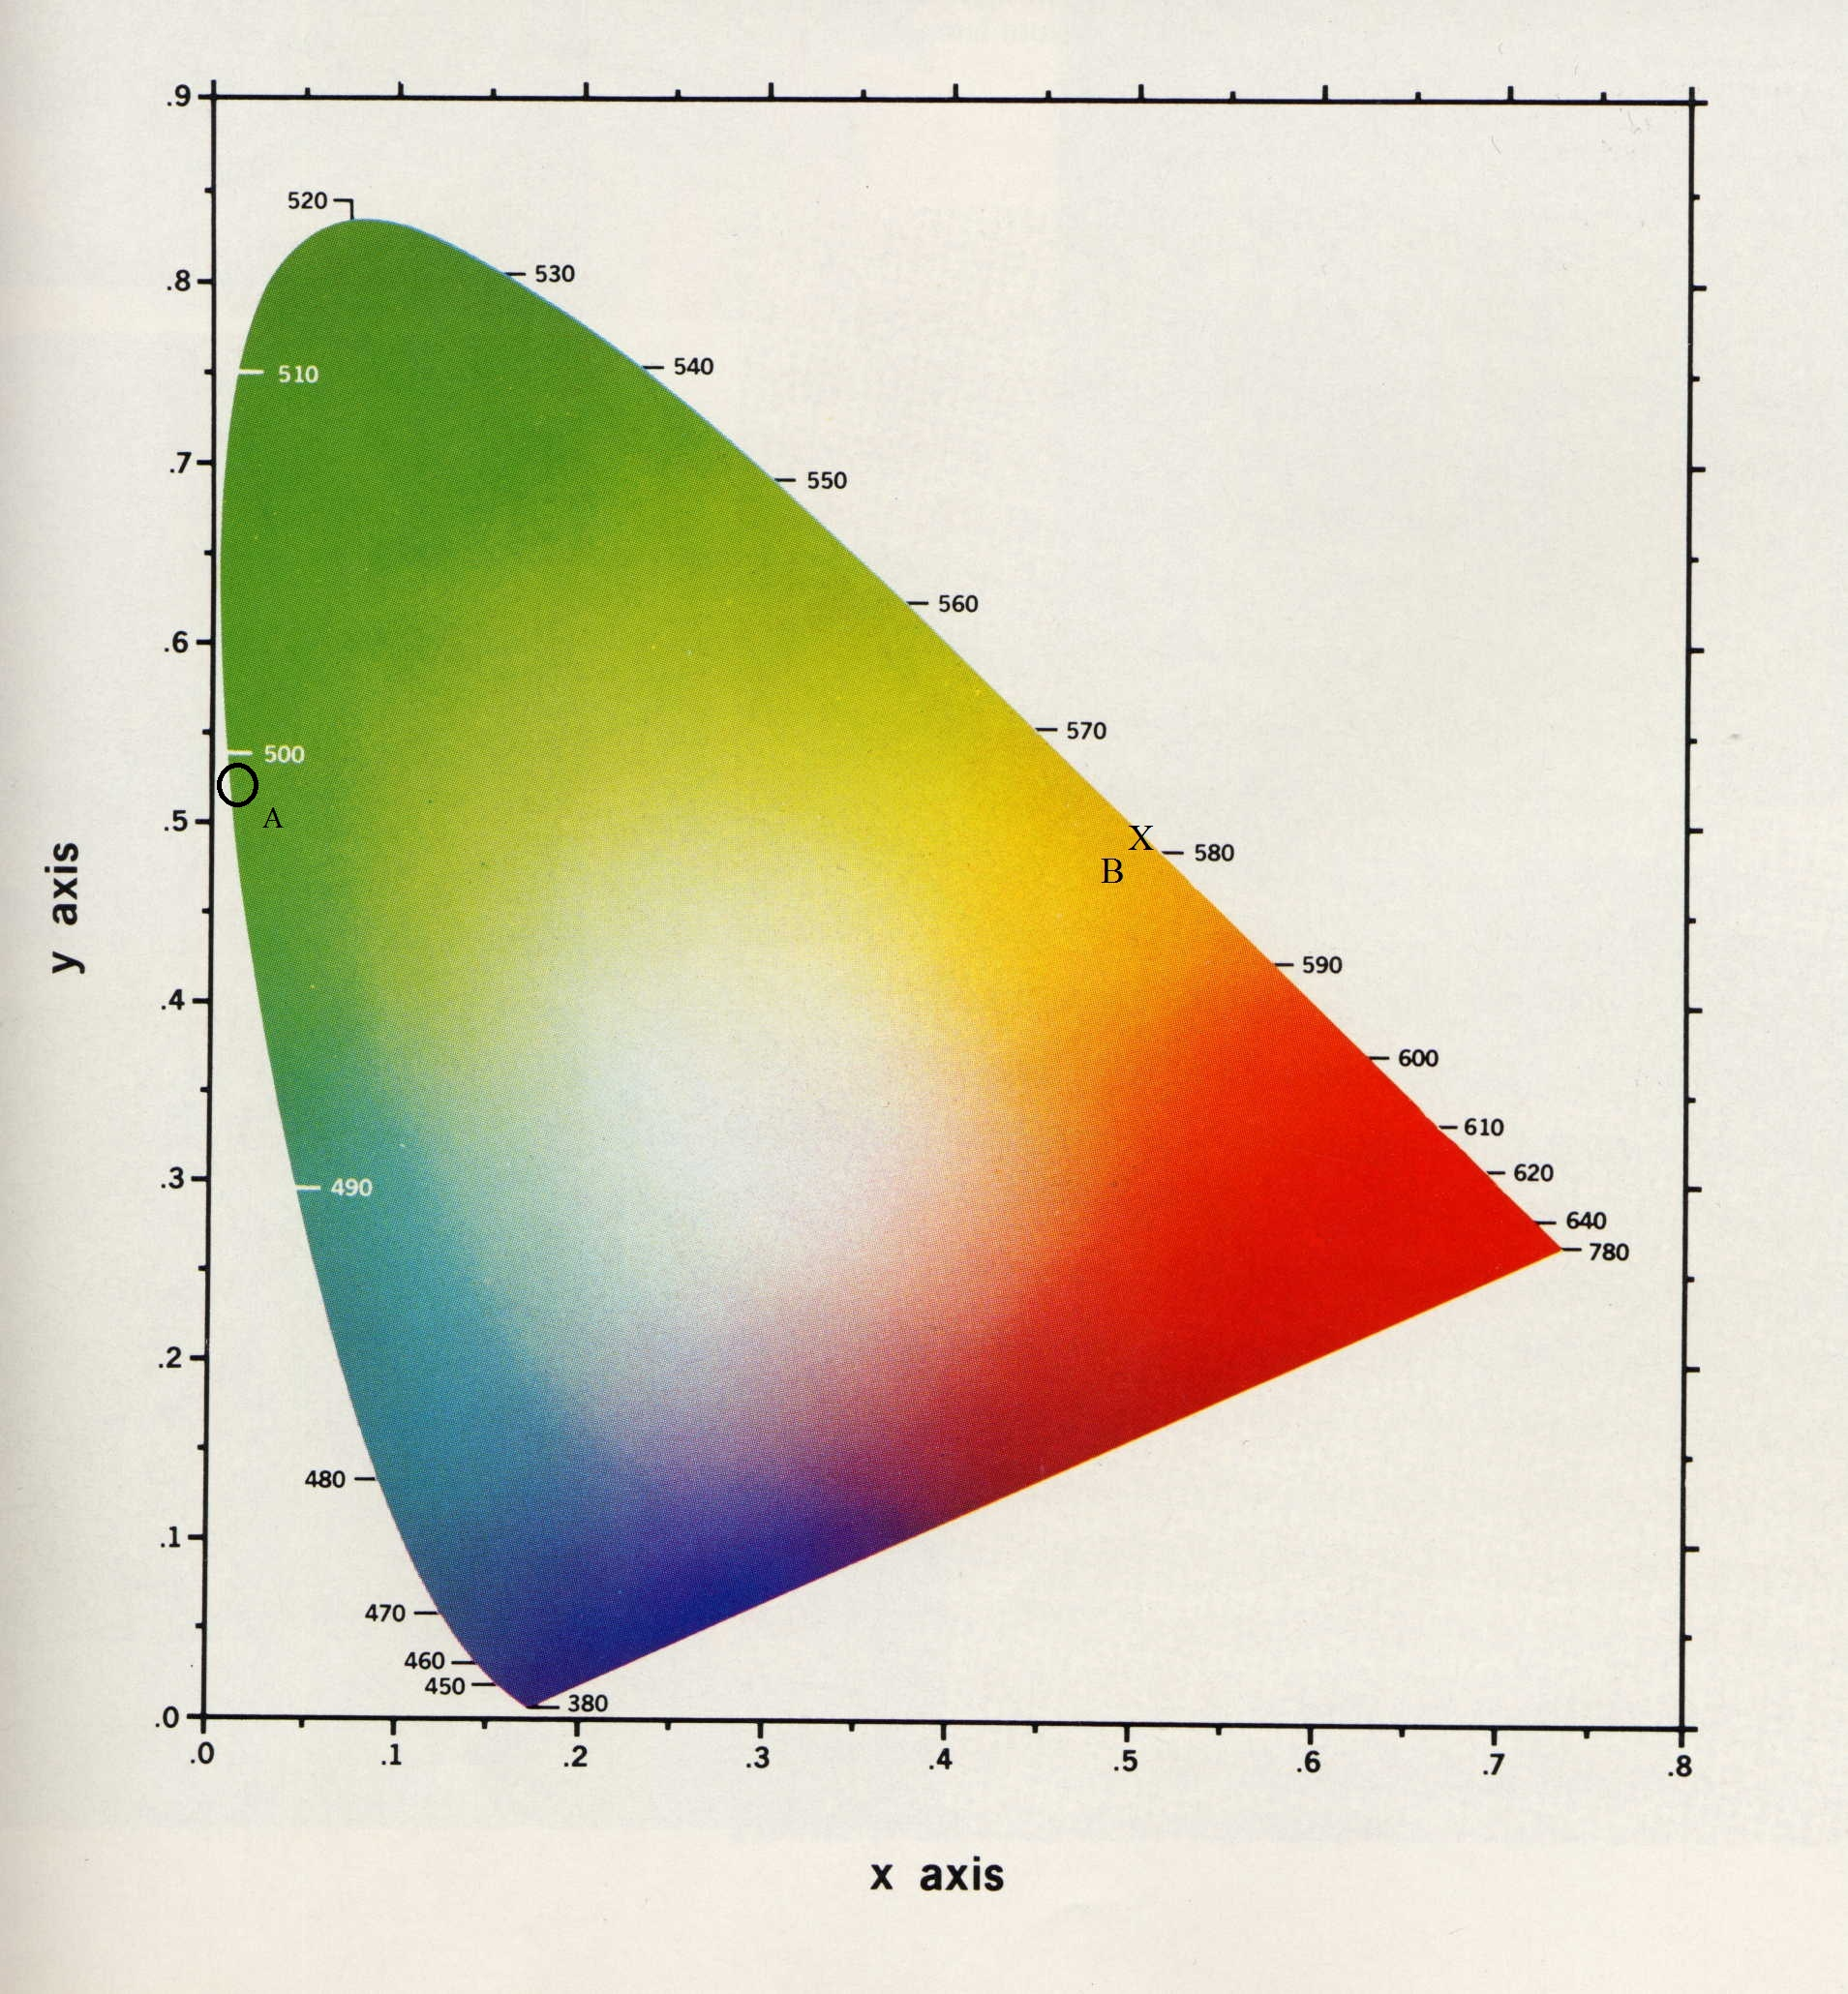
\includegraphics[width=0.4\textwidth]{2d.jpg} 
\end{center}
e) The chromaticity coordinates for color C are :
\begin{gather} 
x_{C} = \frac{X_{A}+X_{B}}{X_{A}+X_{B}+Y_{A}+Y_{B}+Z_{A}+Z_{B}} = \\ = \frac{0.0049+0.9163}{0.0049+0.9163 + 0.323 + 0.870 + 0.272 + 0.0017 } = 0.38 \\
y_{C} = 0.459	\\
z_{C} = 0.114	\\
\end{gather}
f)
\begin{center}
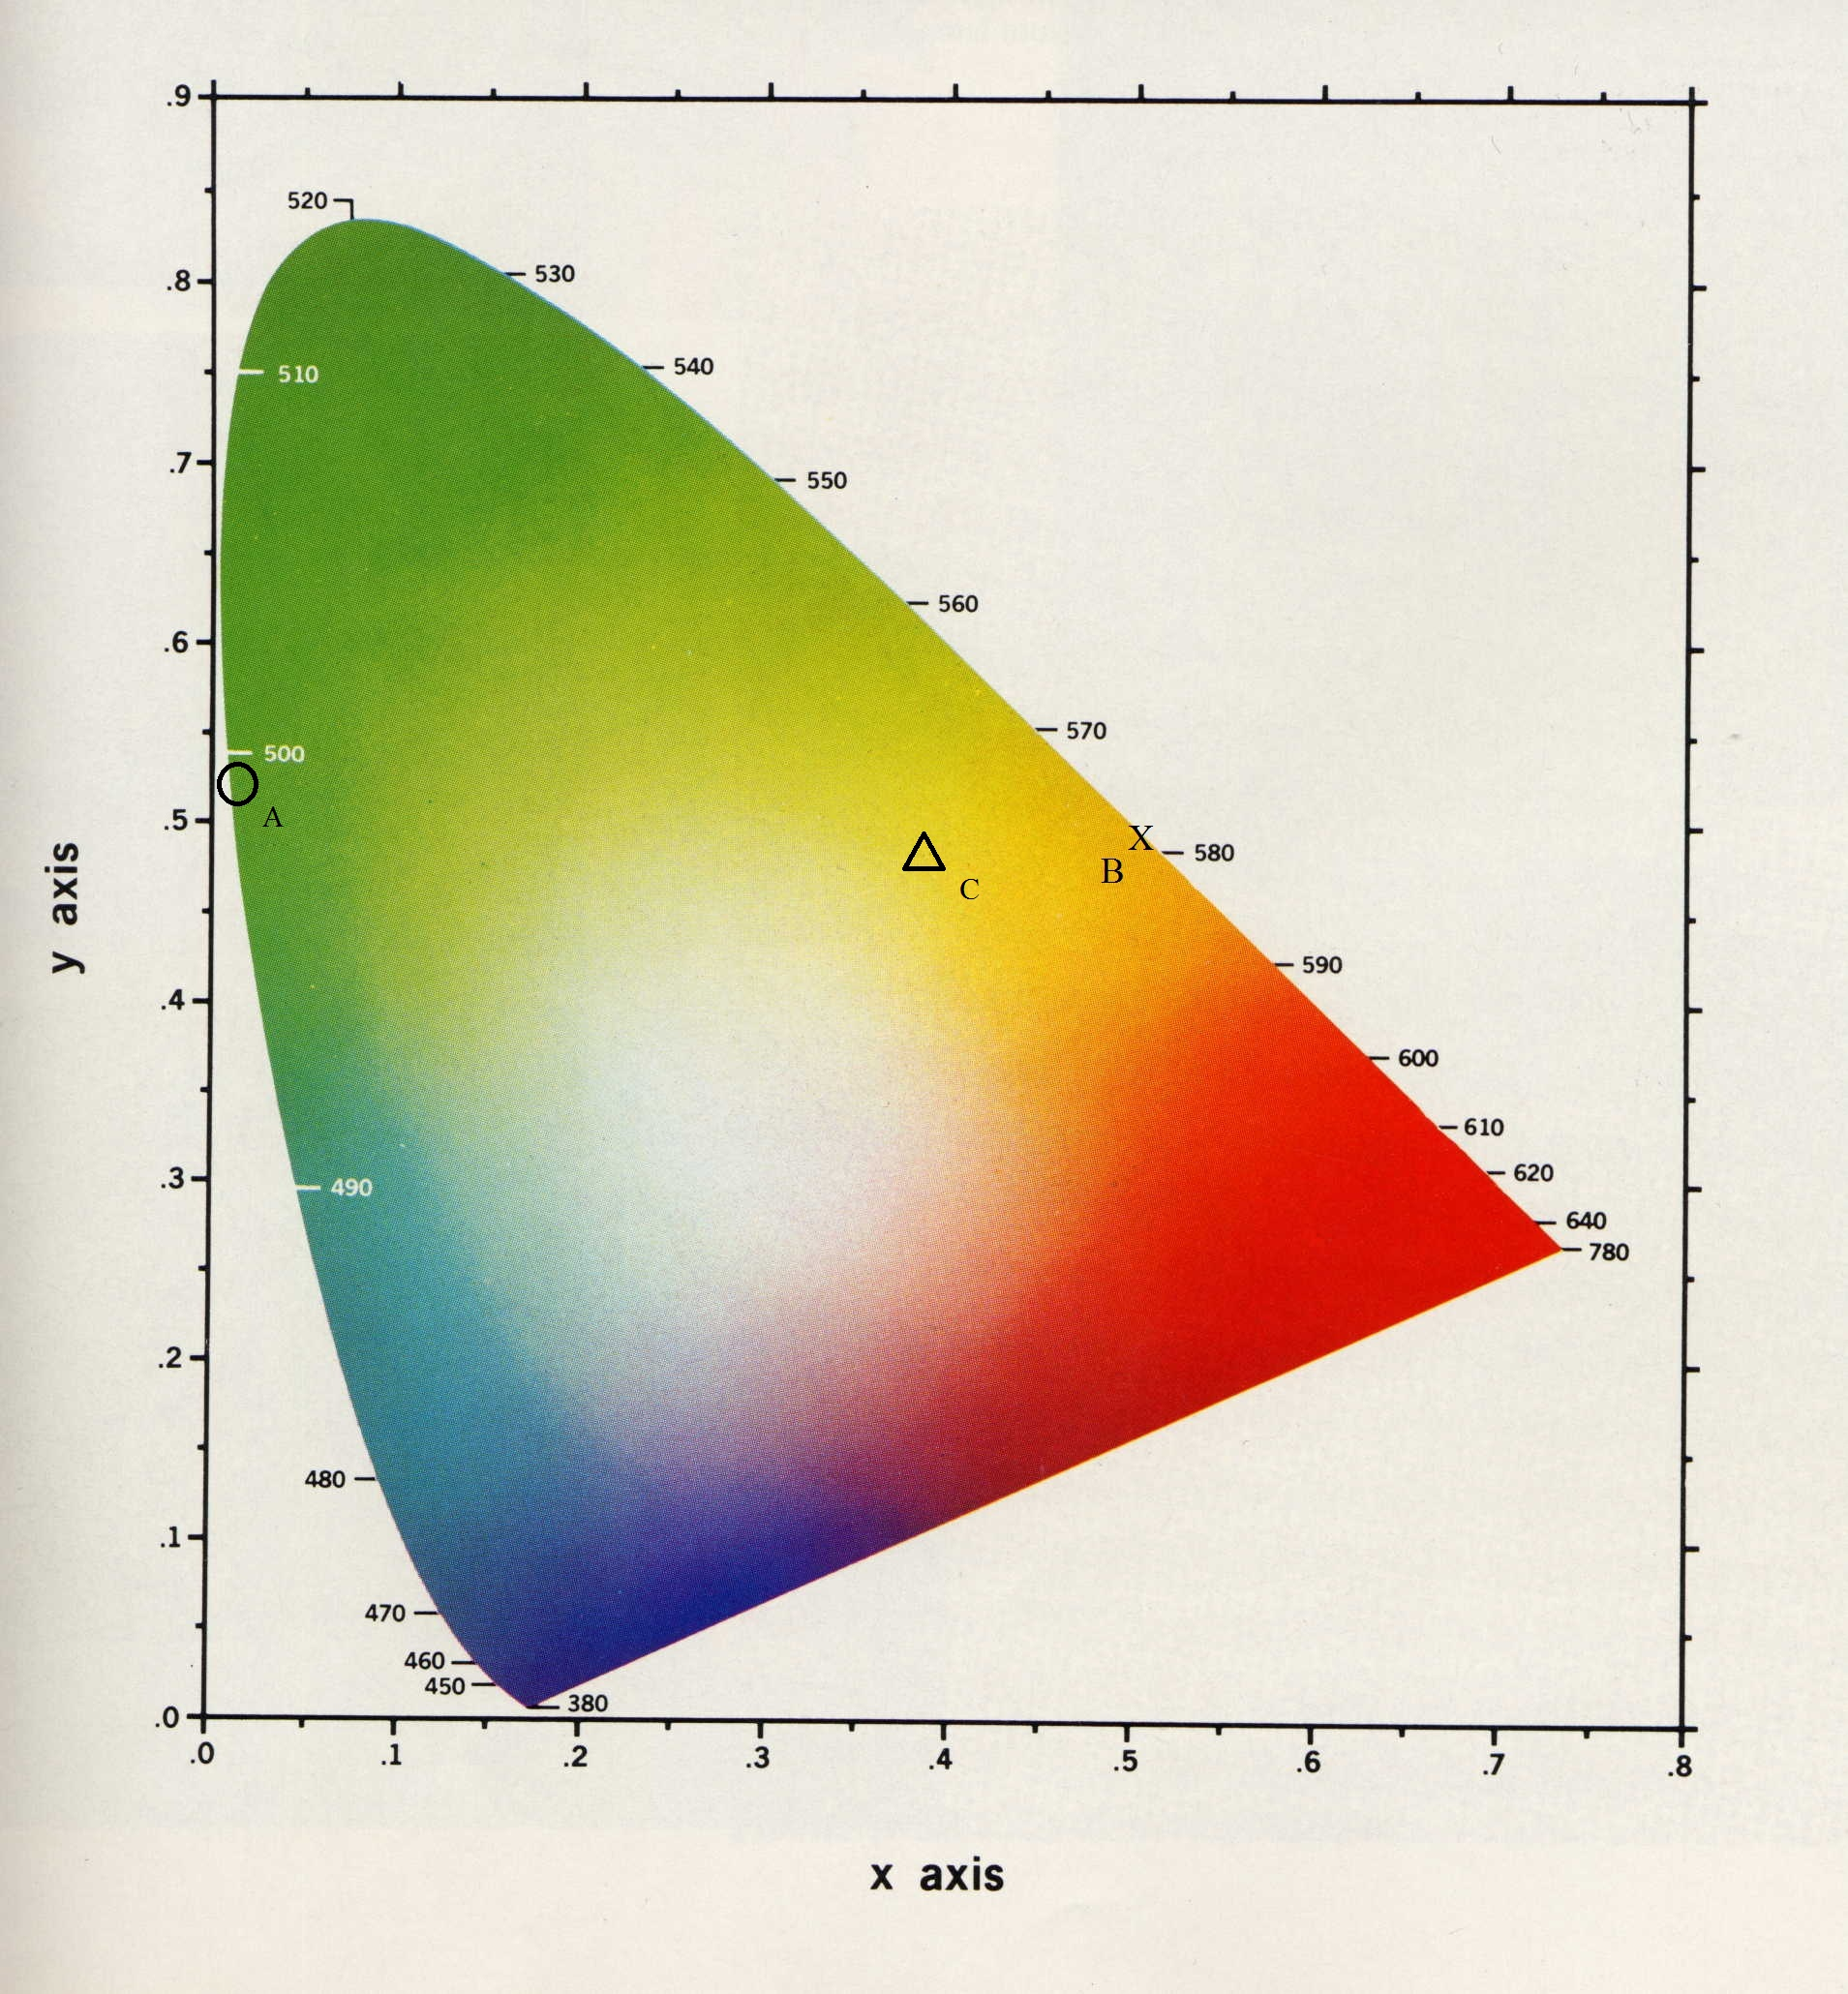
\includegraphics[width=0.4\textwidth]{2f.jpg} 
\end{center}
g) In the case of normalized colors xyz it is invariant to intensity, whereas in the XYZ system it they will change with K. A, B and C remain the same. \\\\
h) 
\begin{gather}  
x_{L} = \frac{X_{L}}{X_{L}+Y_{L}+Z_{L}} = \frac{98.04}{98.04+100+118.12} = 0.31 \\
y_{L} = 0.316 \\
z_{L} = 0.373 \\
\end{gather}
\begin{center}
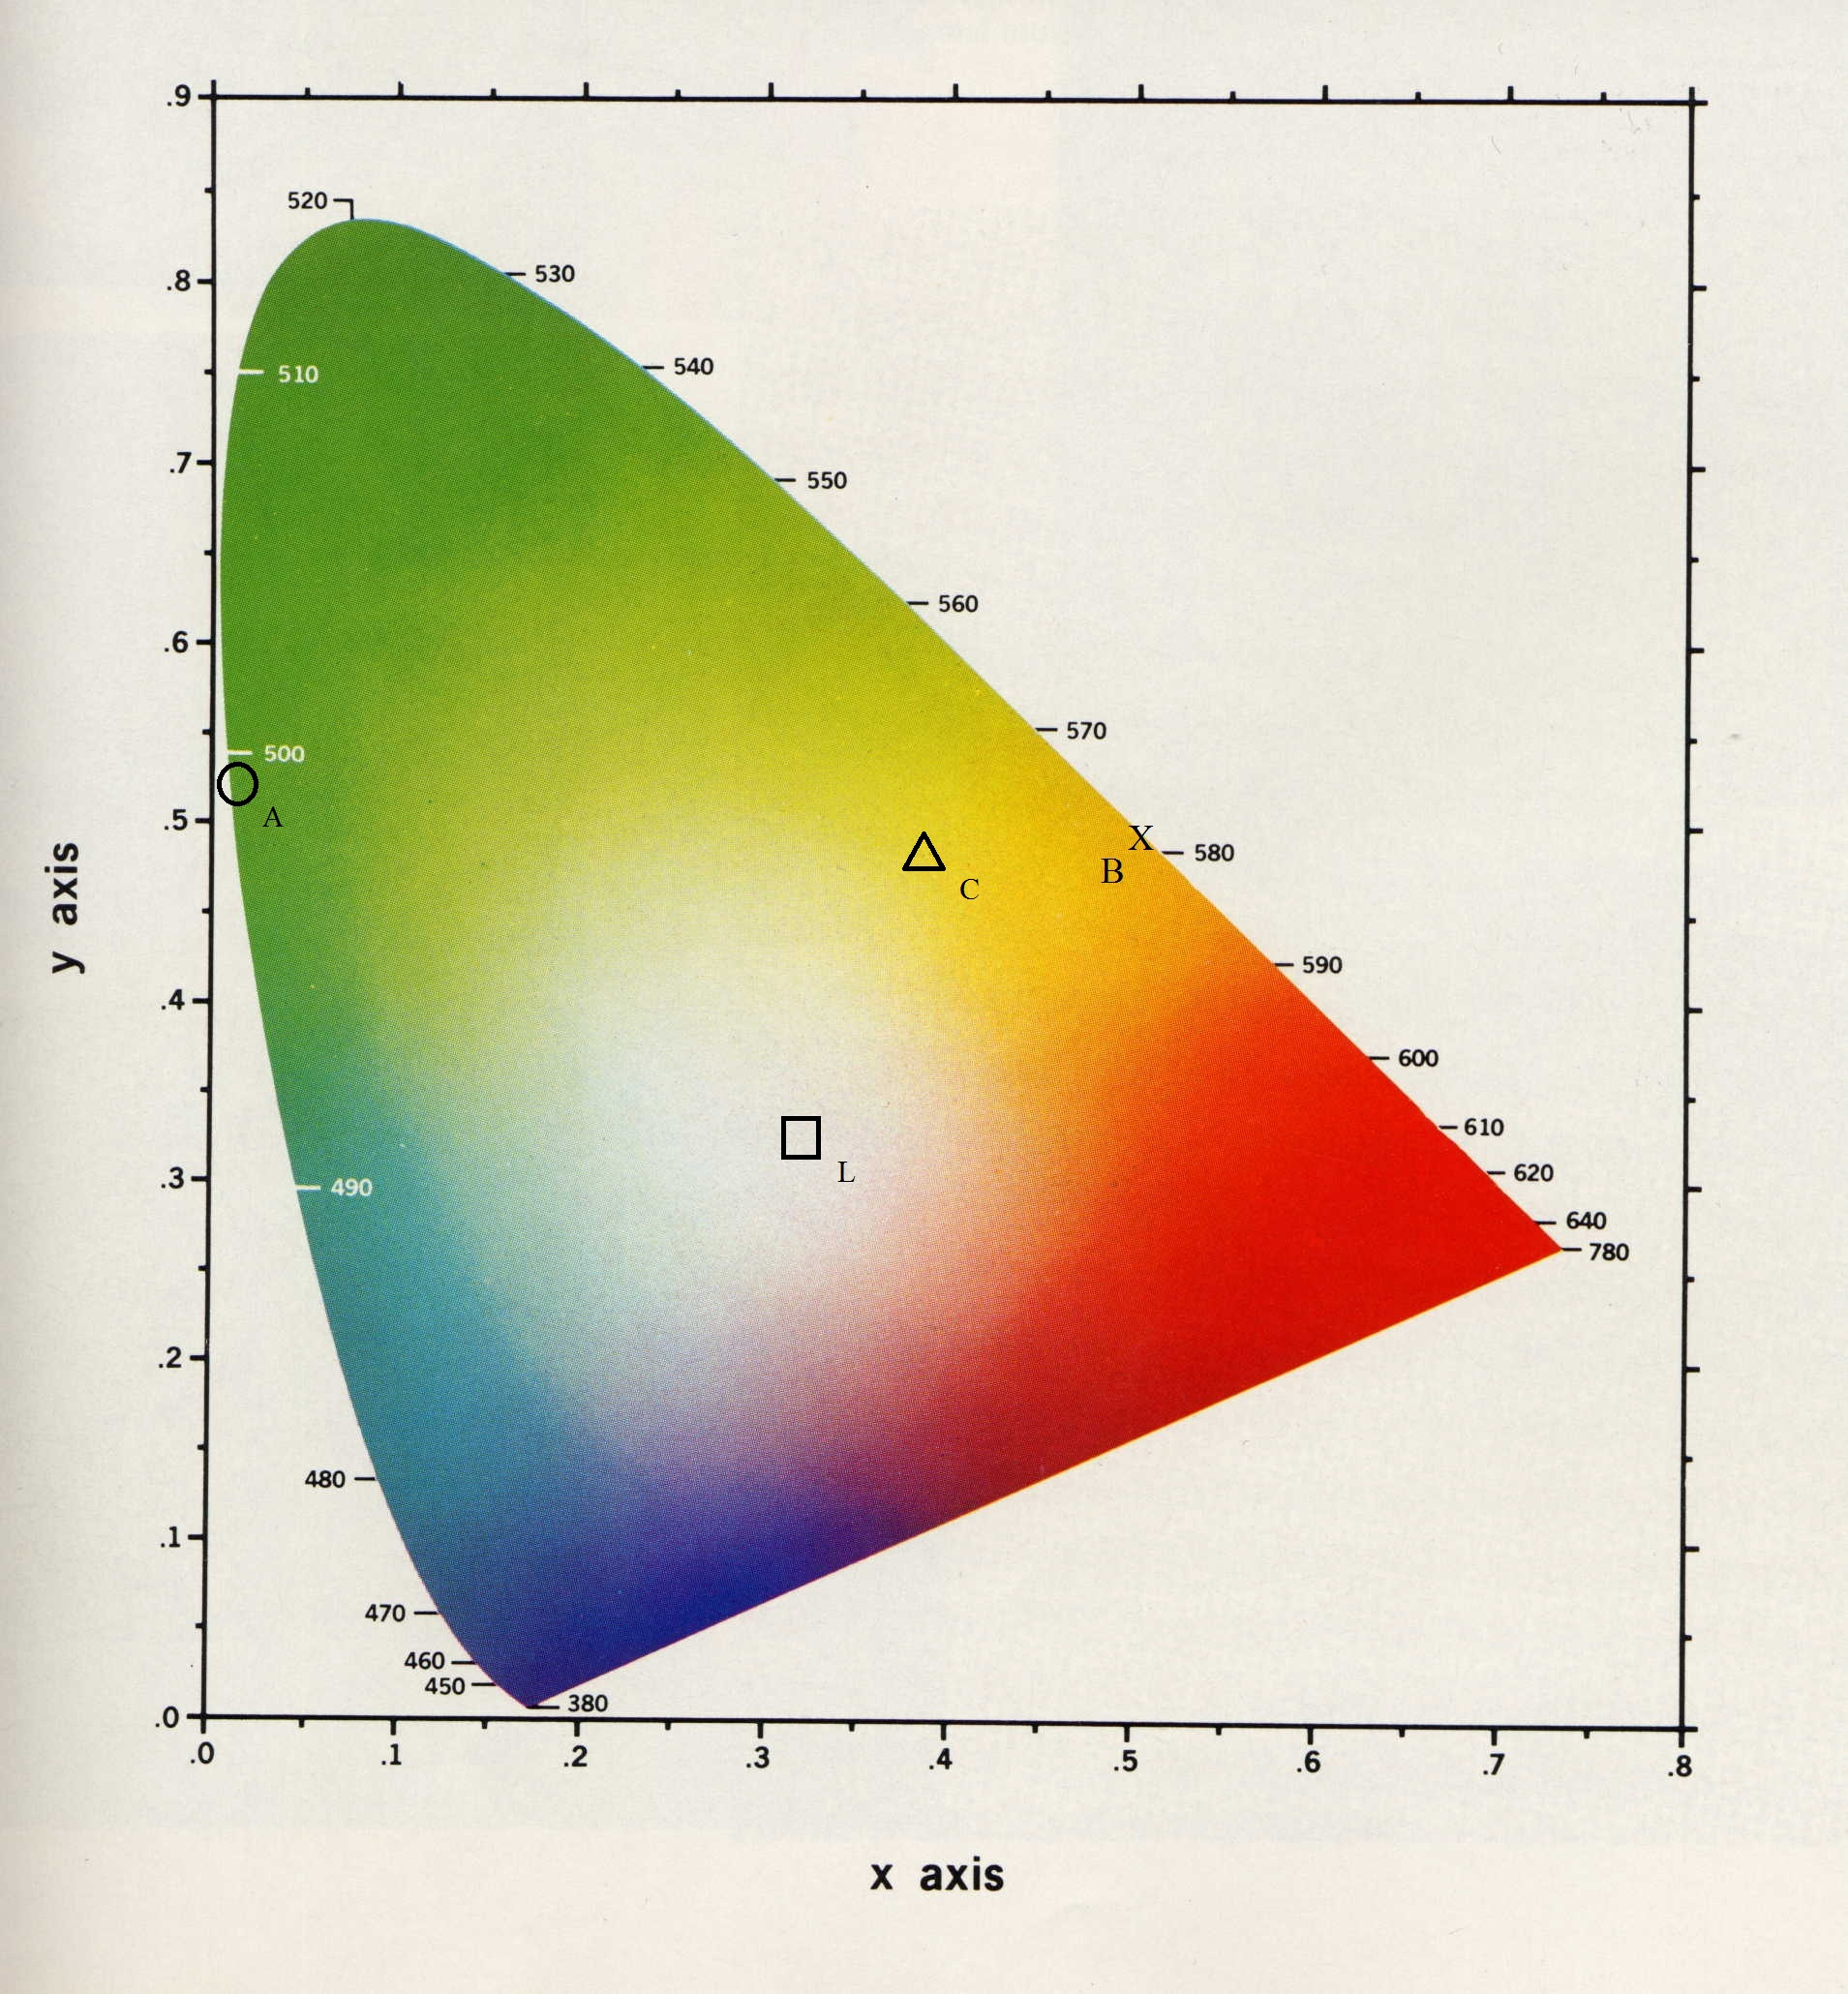
\includegraphics[width=0.4\textwidth]{2h.jpg}
\end{center}
i)
\begin{center}
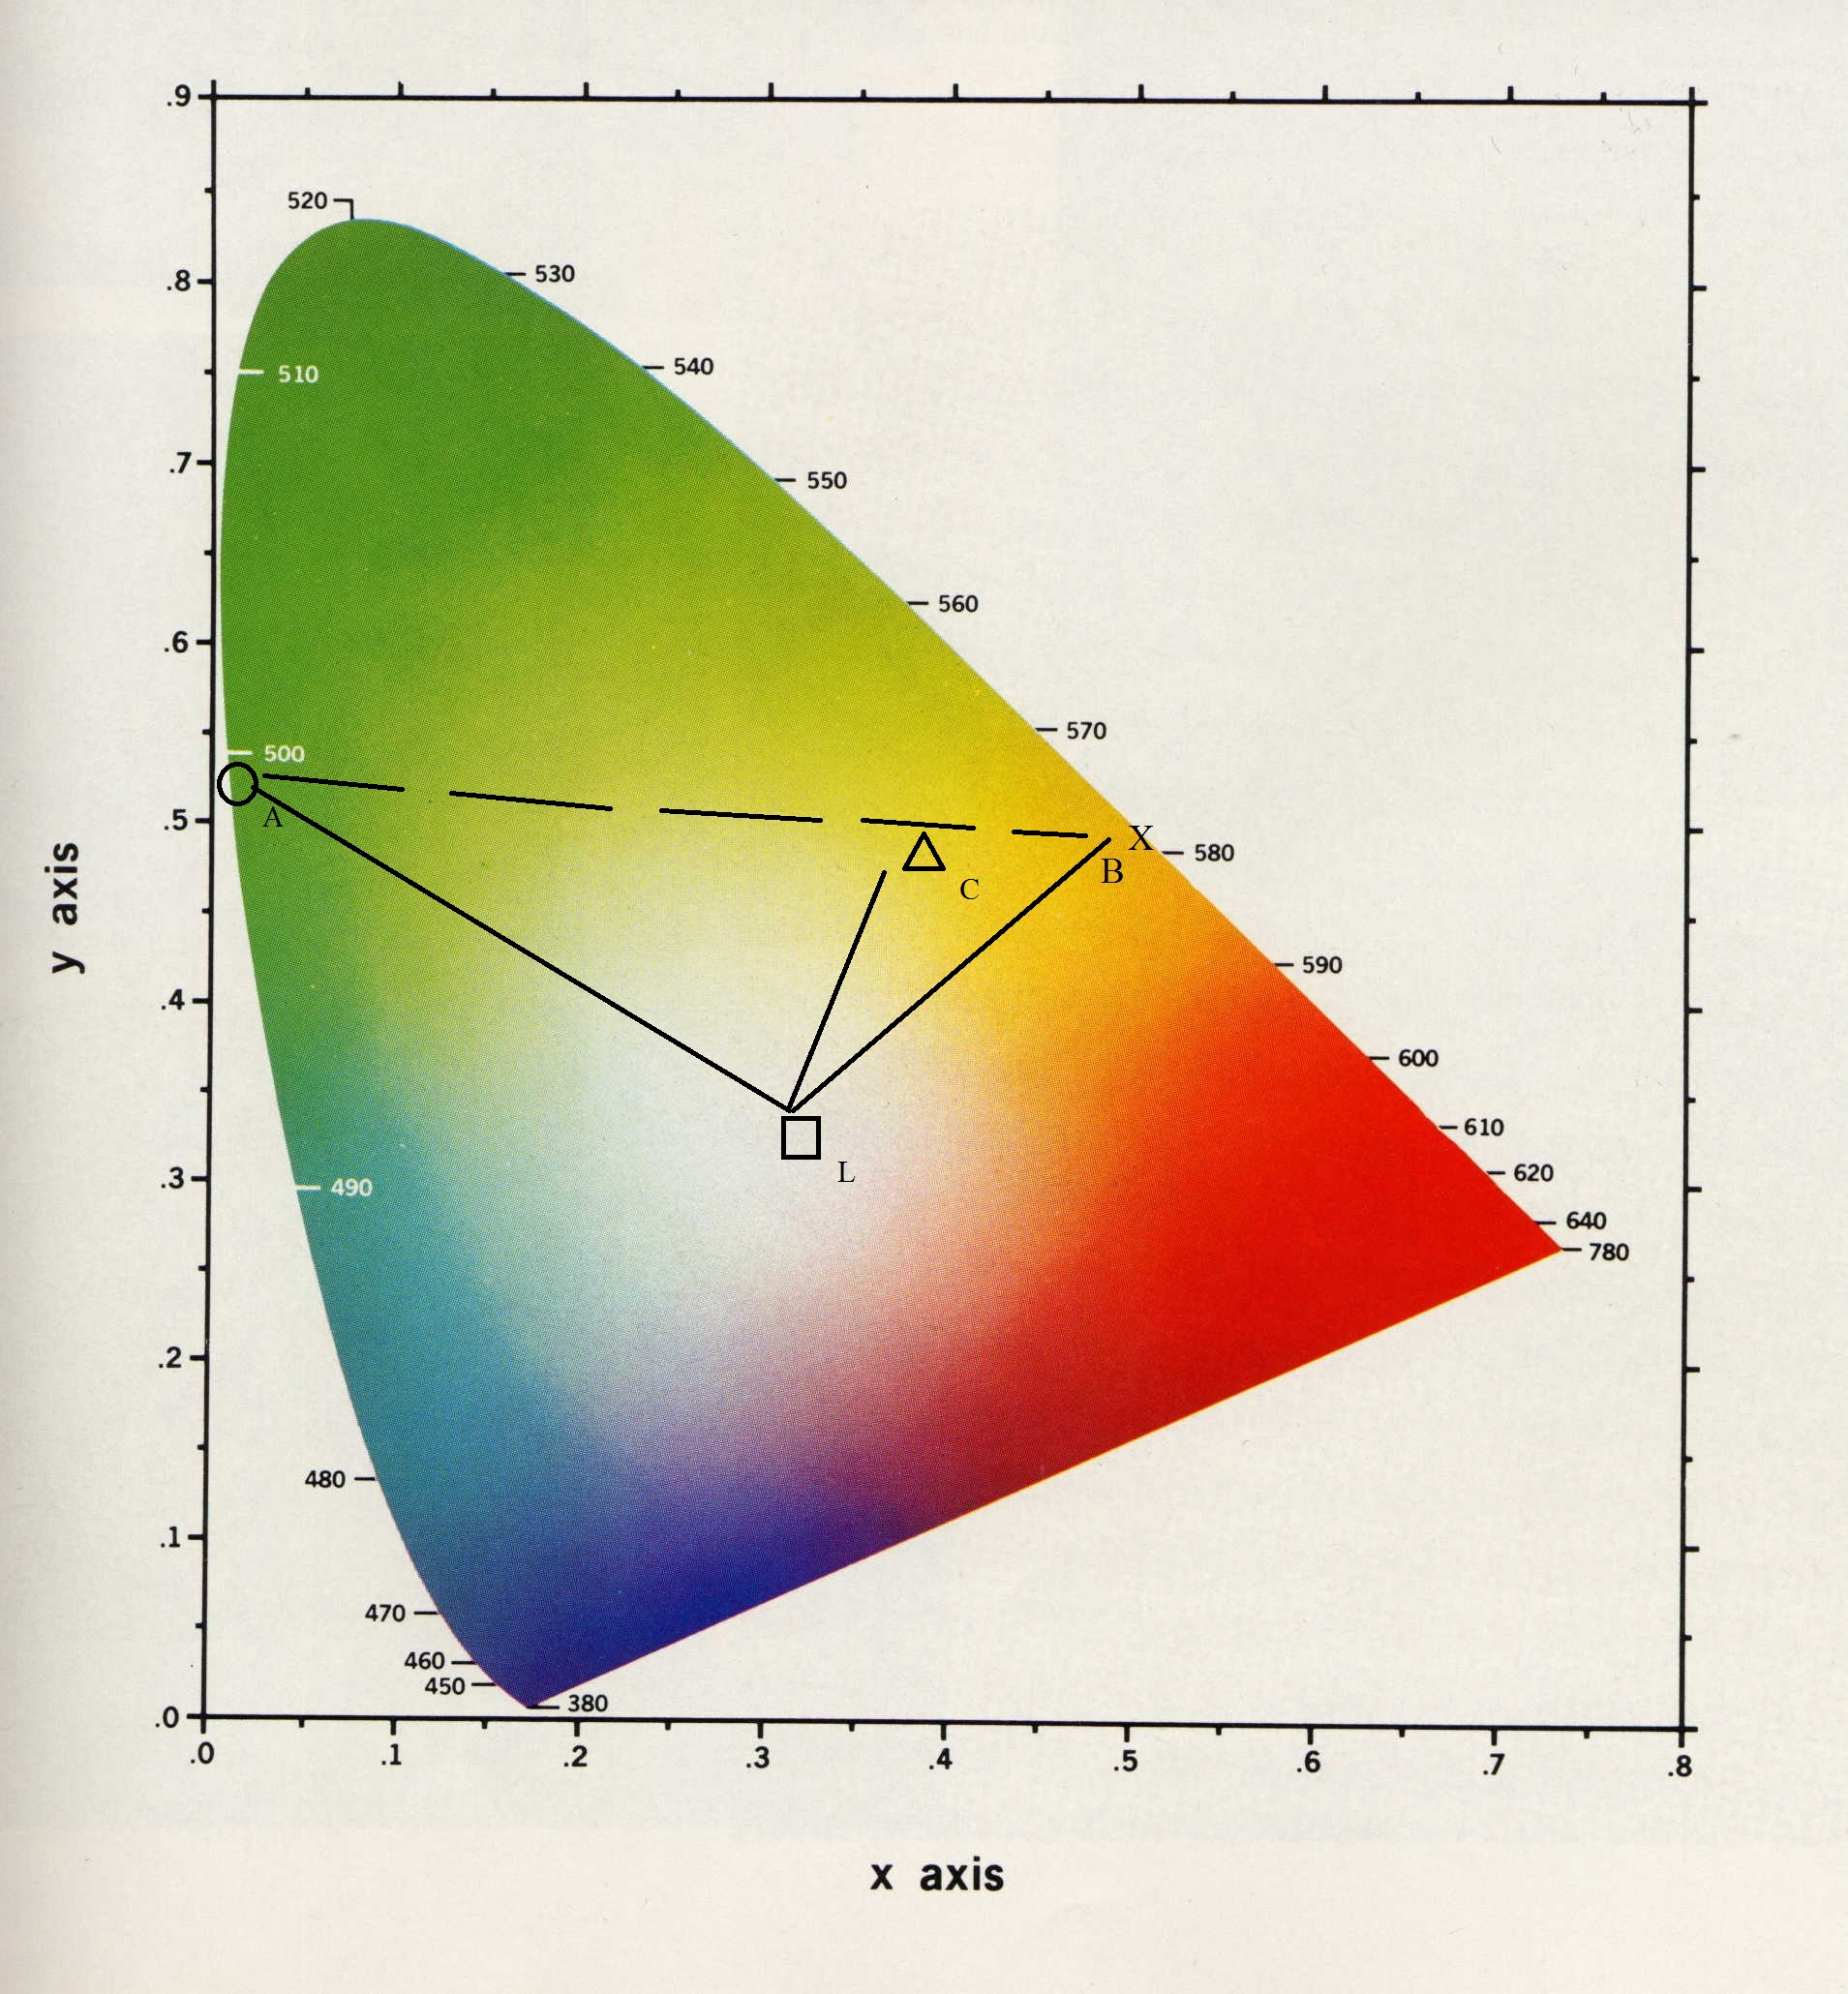
\includegraphics[width=0.4\textwidth]{2i.jpg}
\end{center}
j) Hue = 550nm
\begin{center}
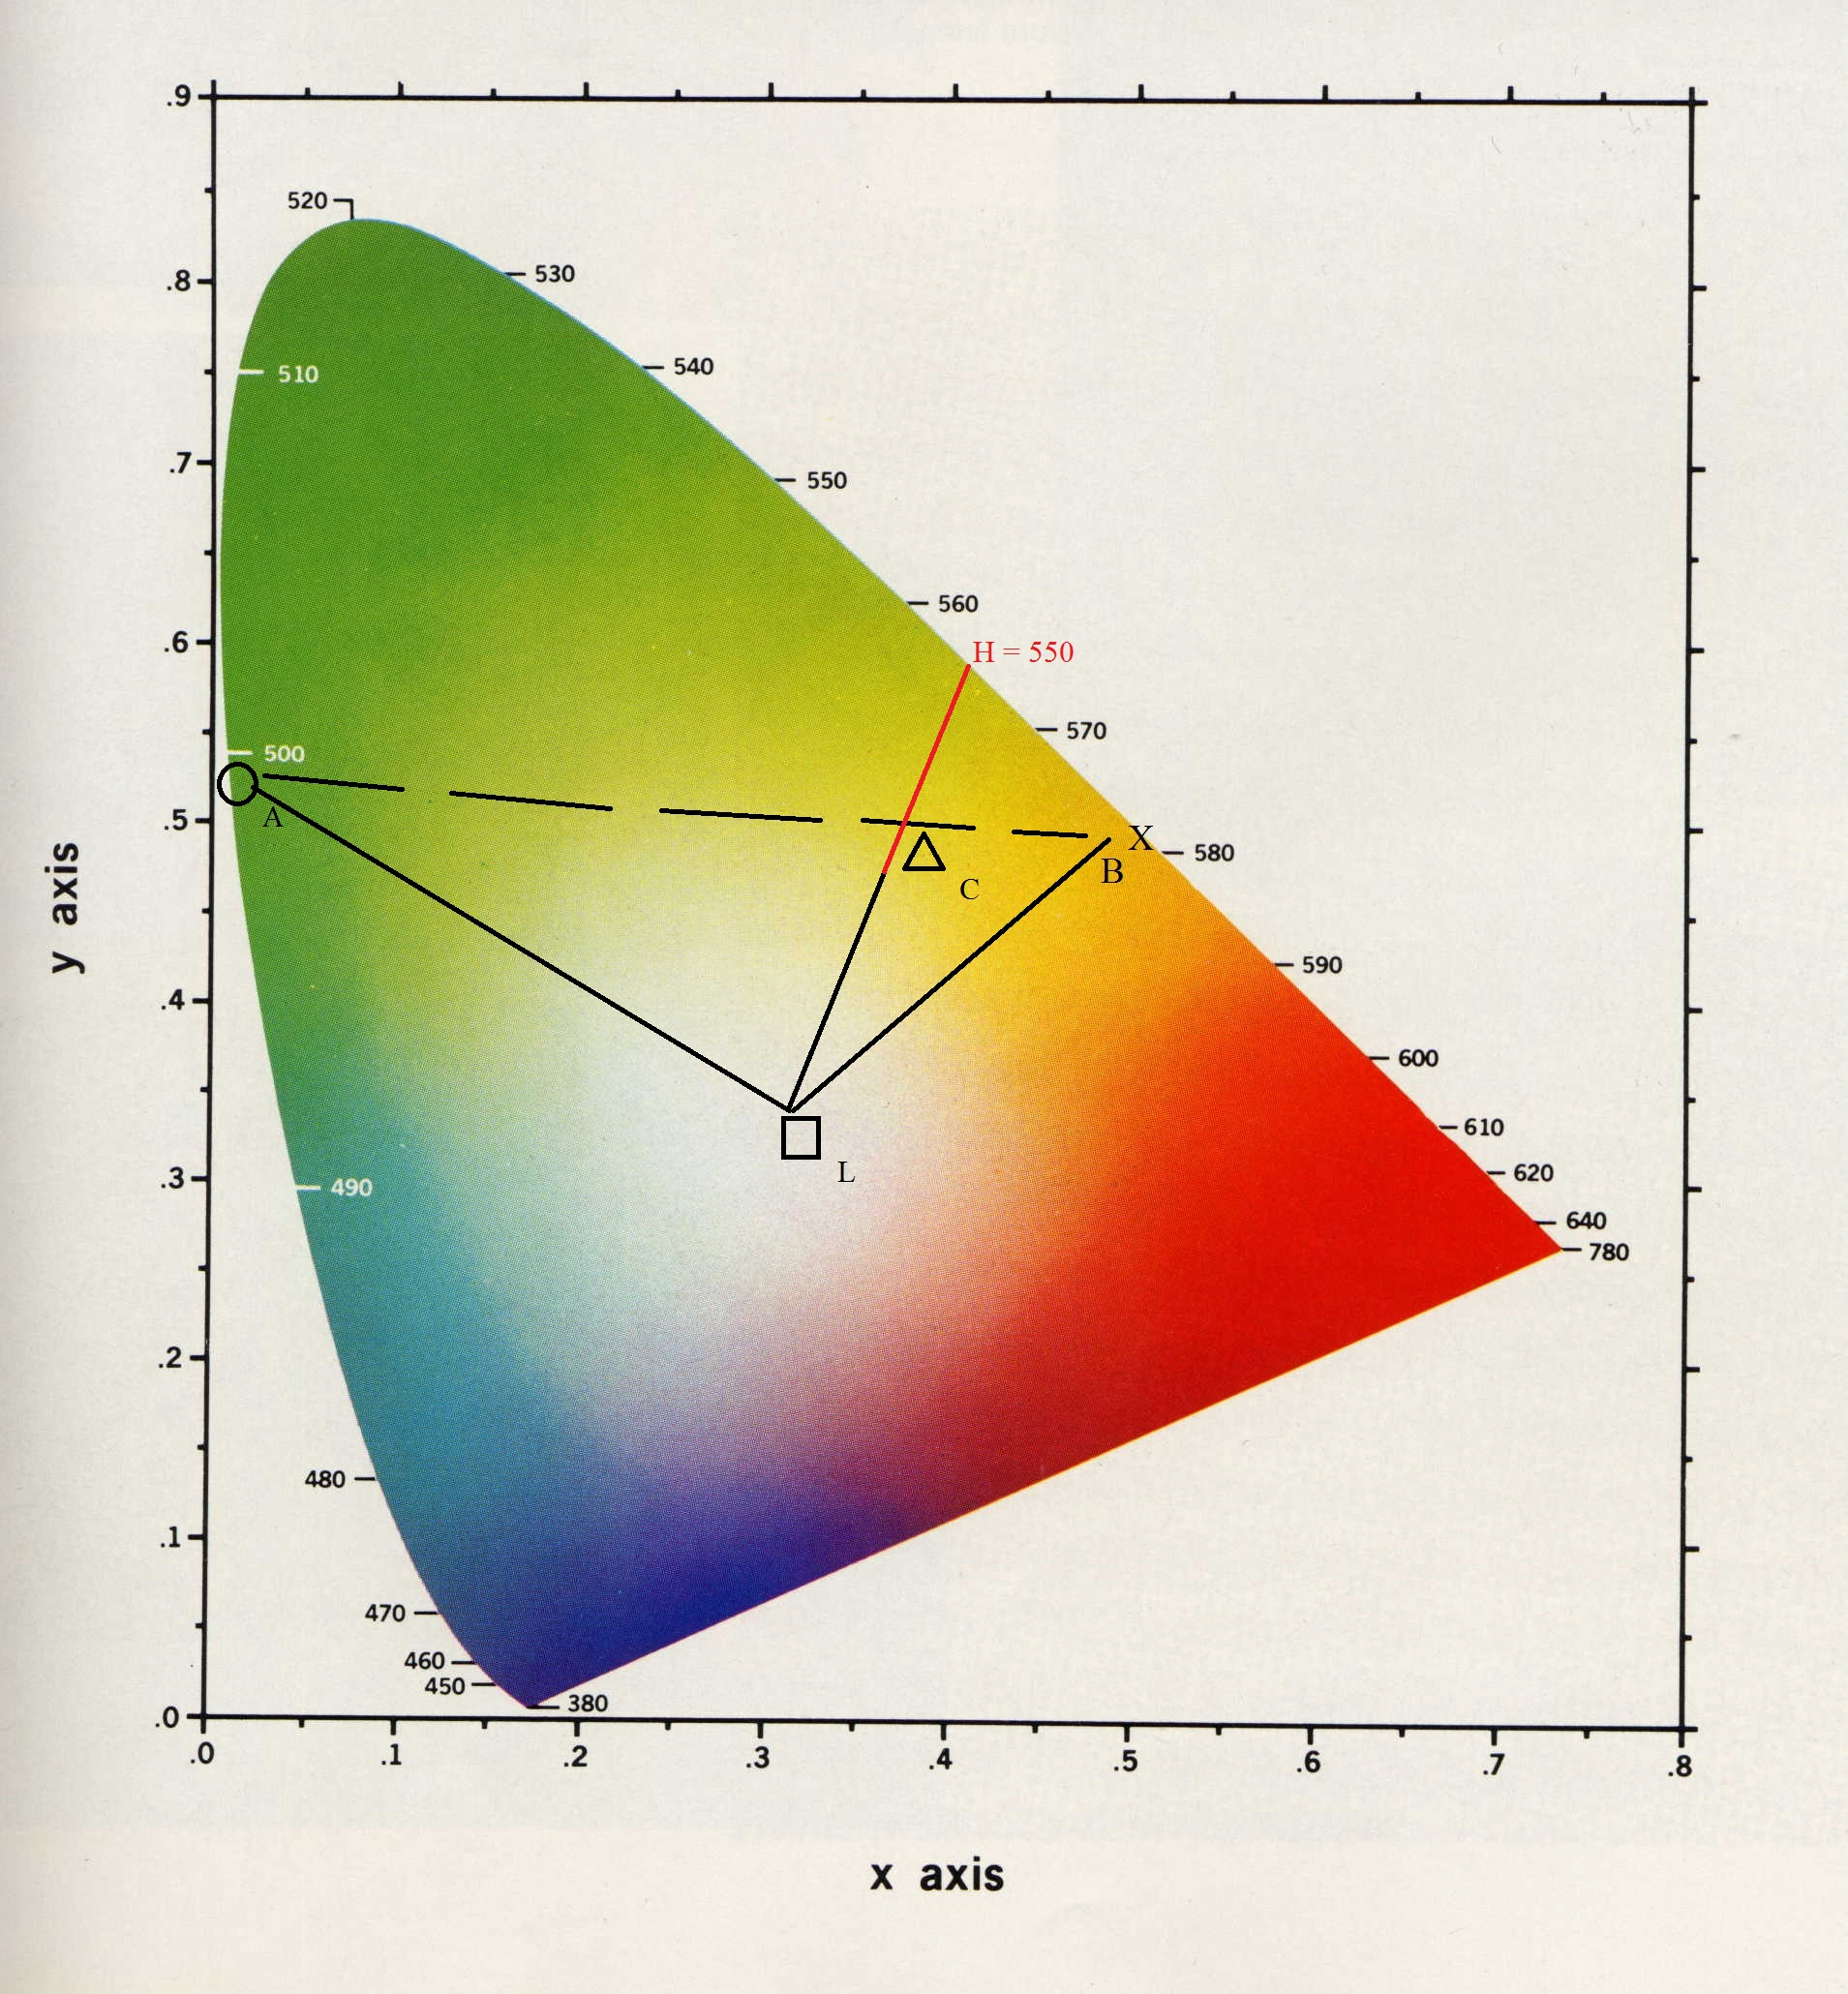
\includegraphics[width=0.4\textwidth]{2j.jpg}
\end{center}
k) Reminder: the closer to the edge the more saturated a color is.
\begin{gather}  
S_{A} = S{B} > S_{C} > S_{L} \\
\end{gather}
l)Complementary colors:
A does not have a complementary color because it is not a spectral color.
\begin{center}
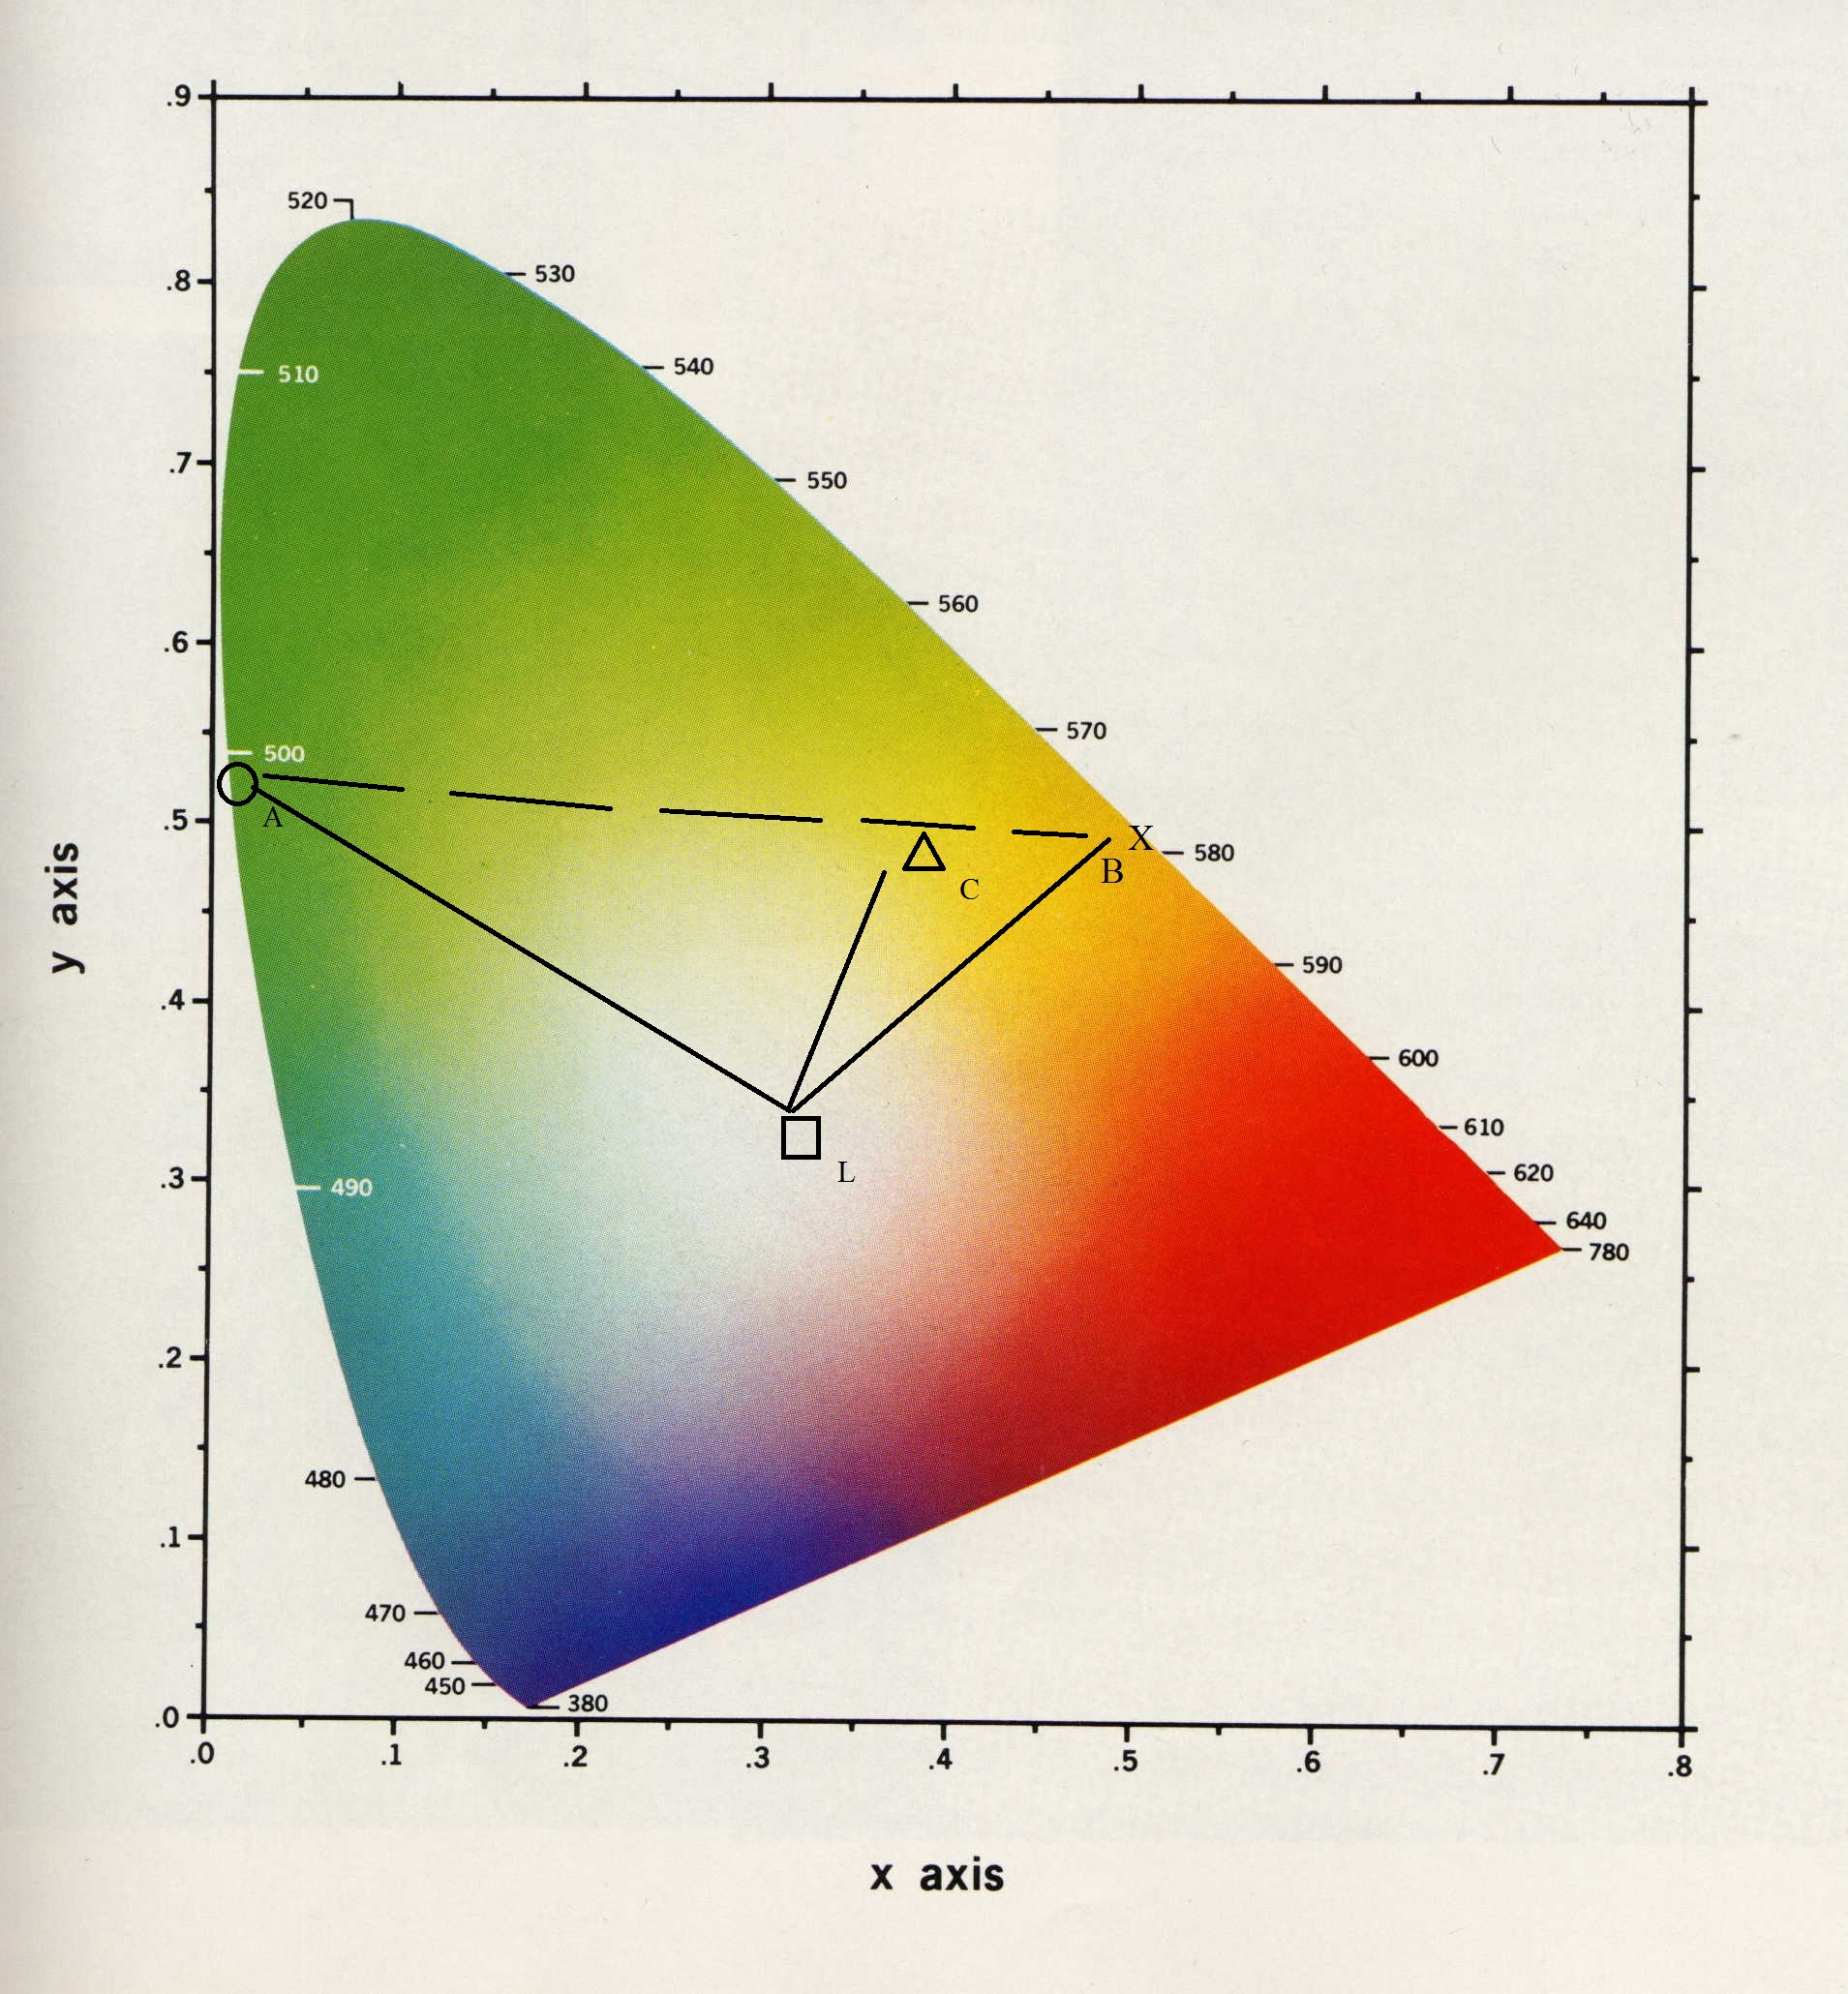
\includegraphics[width=0.4\textwidth]{2l.jpg}
\end{center}
m)
\begin{center}
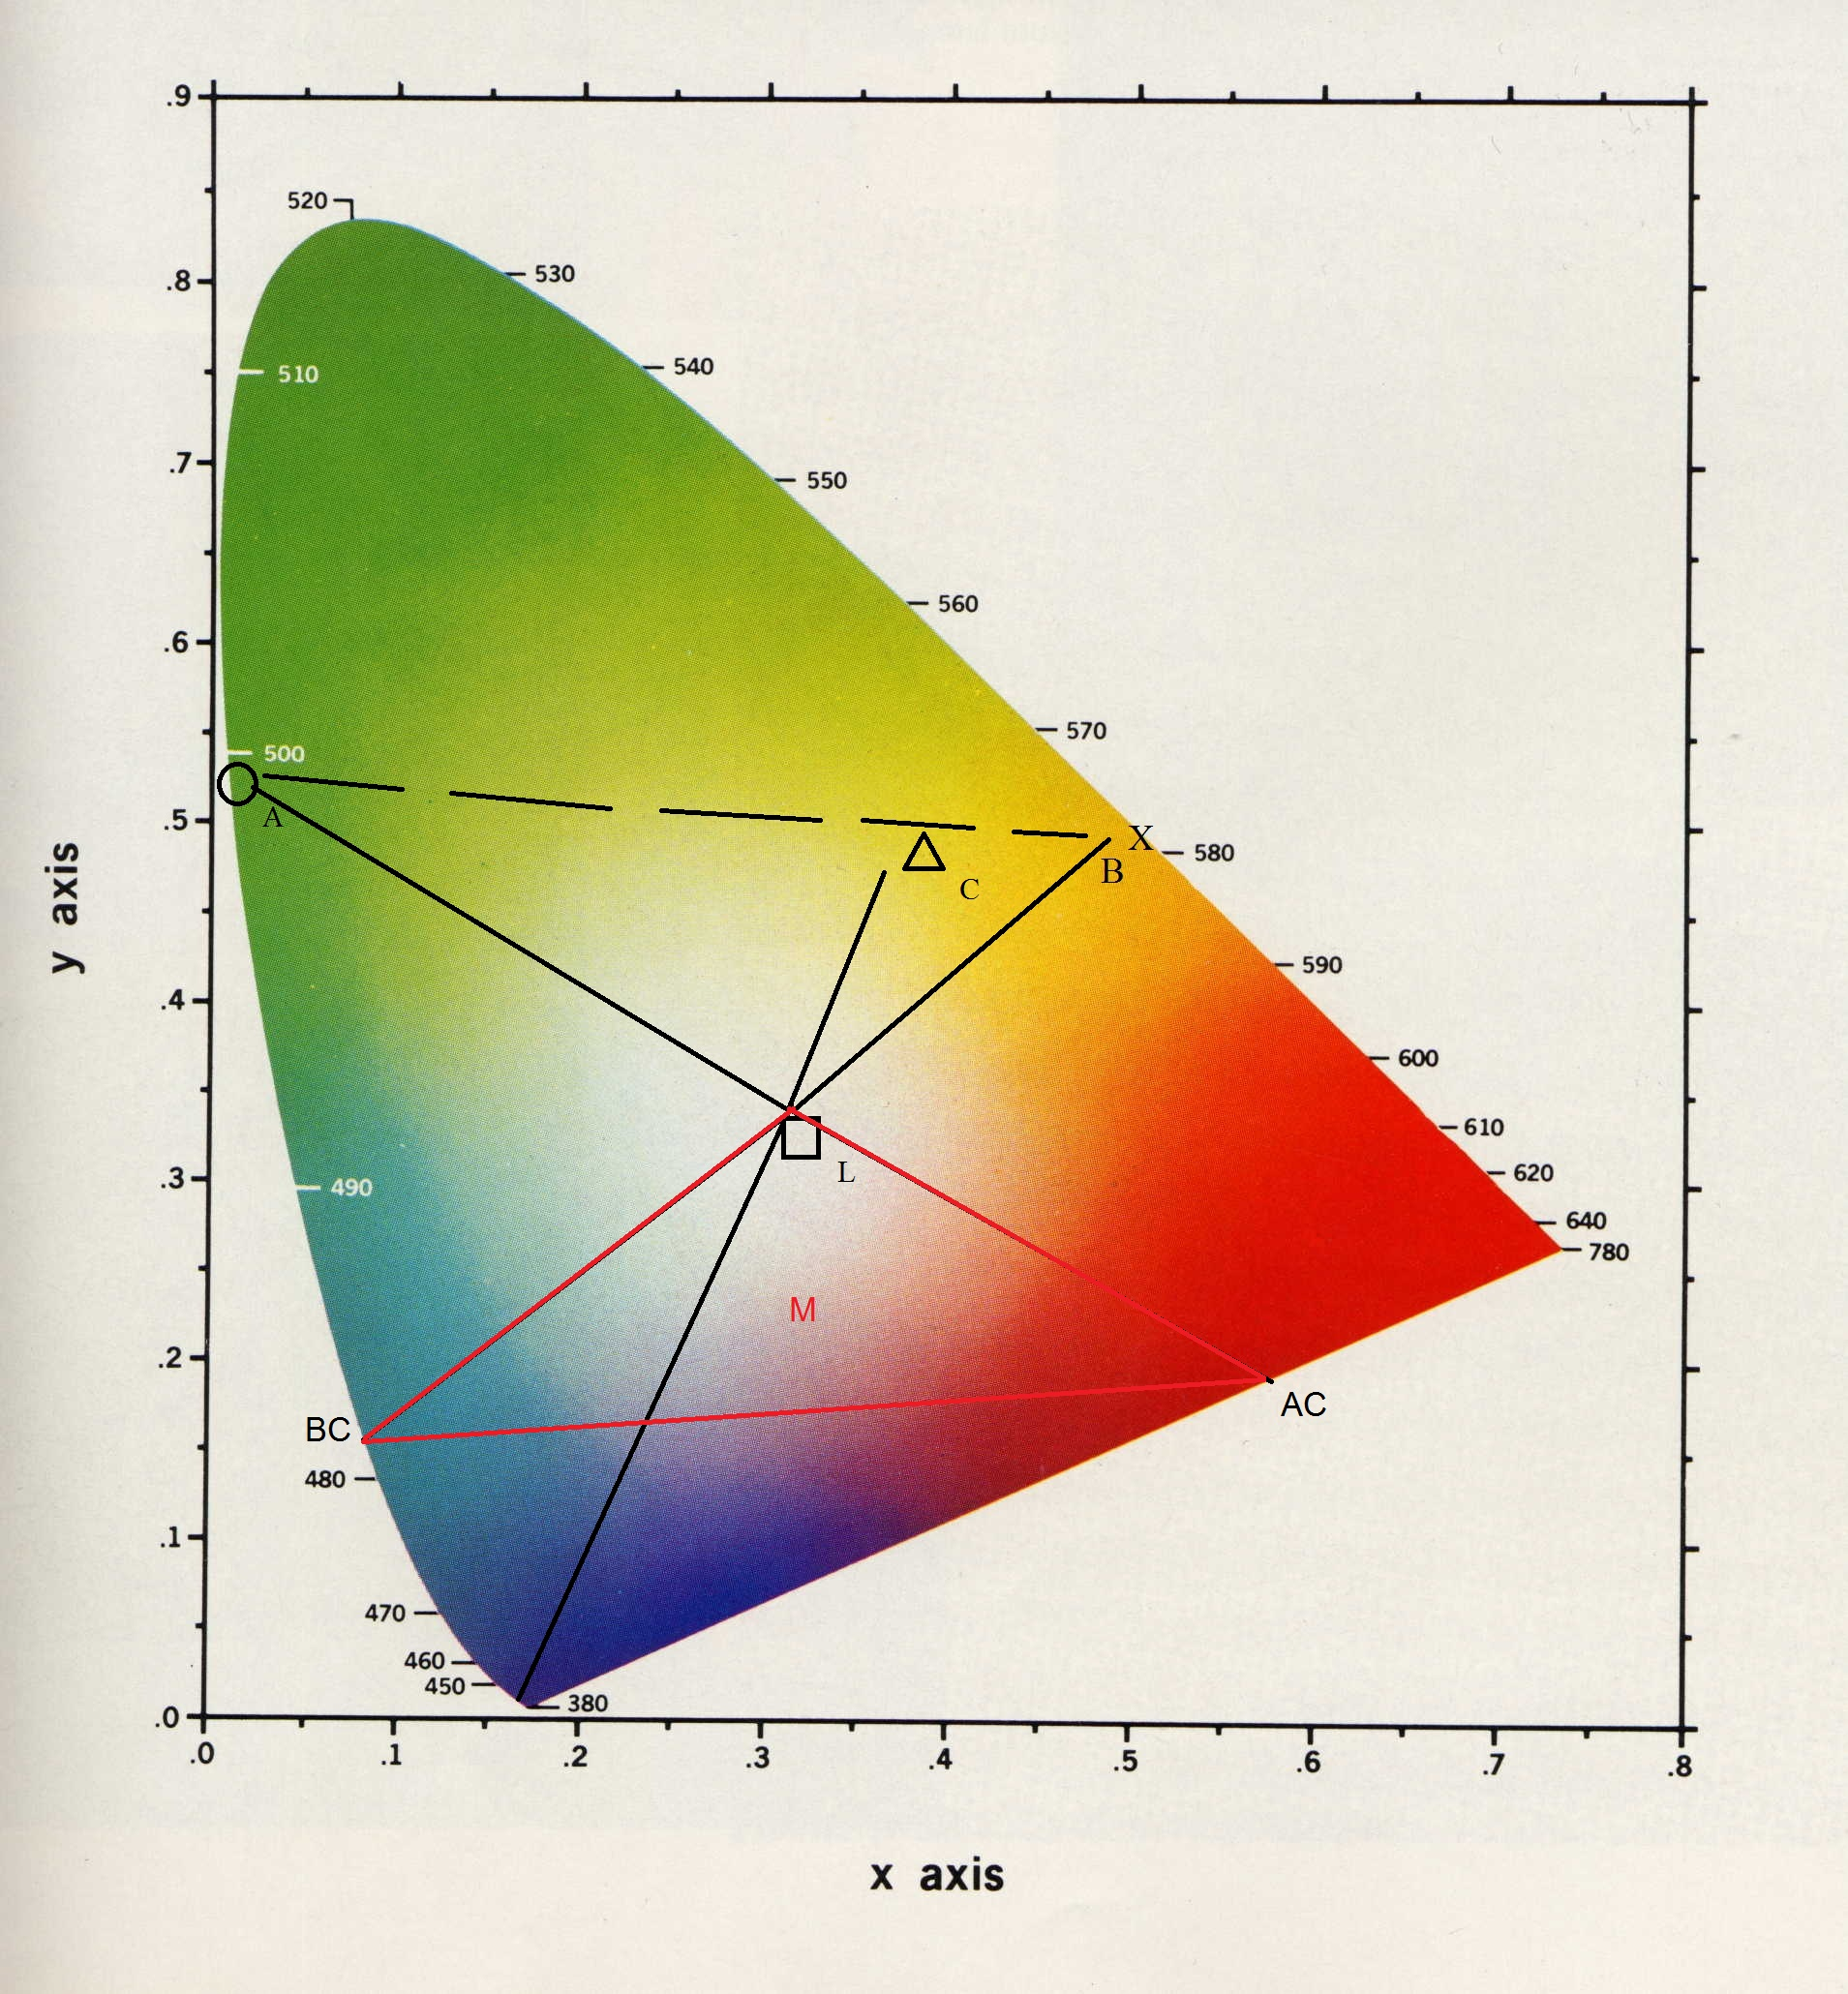
\includegraphics[width=0.4\textwidth]{2m.jpg}
\end{center}
n)
Dominant wavelength is 510nm. Approximated position is (look up values in the table):
\begin{gather}  
x = 0.013 //
y = 0.75
\end{gather}
\begin{center}
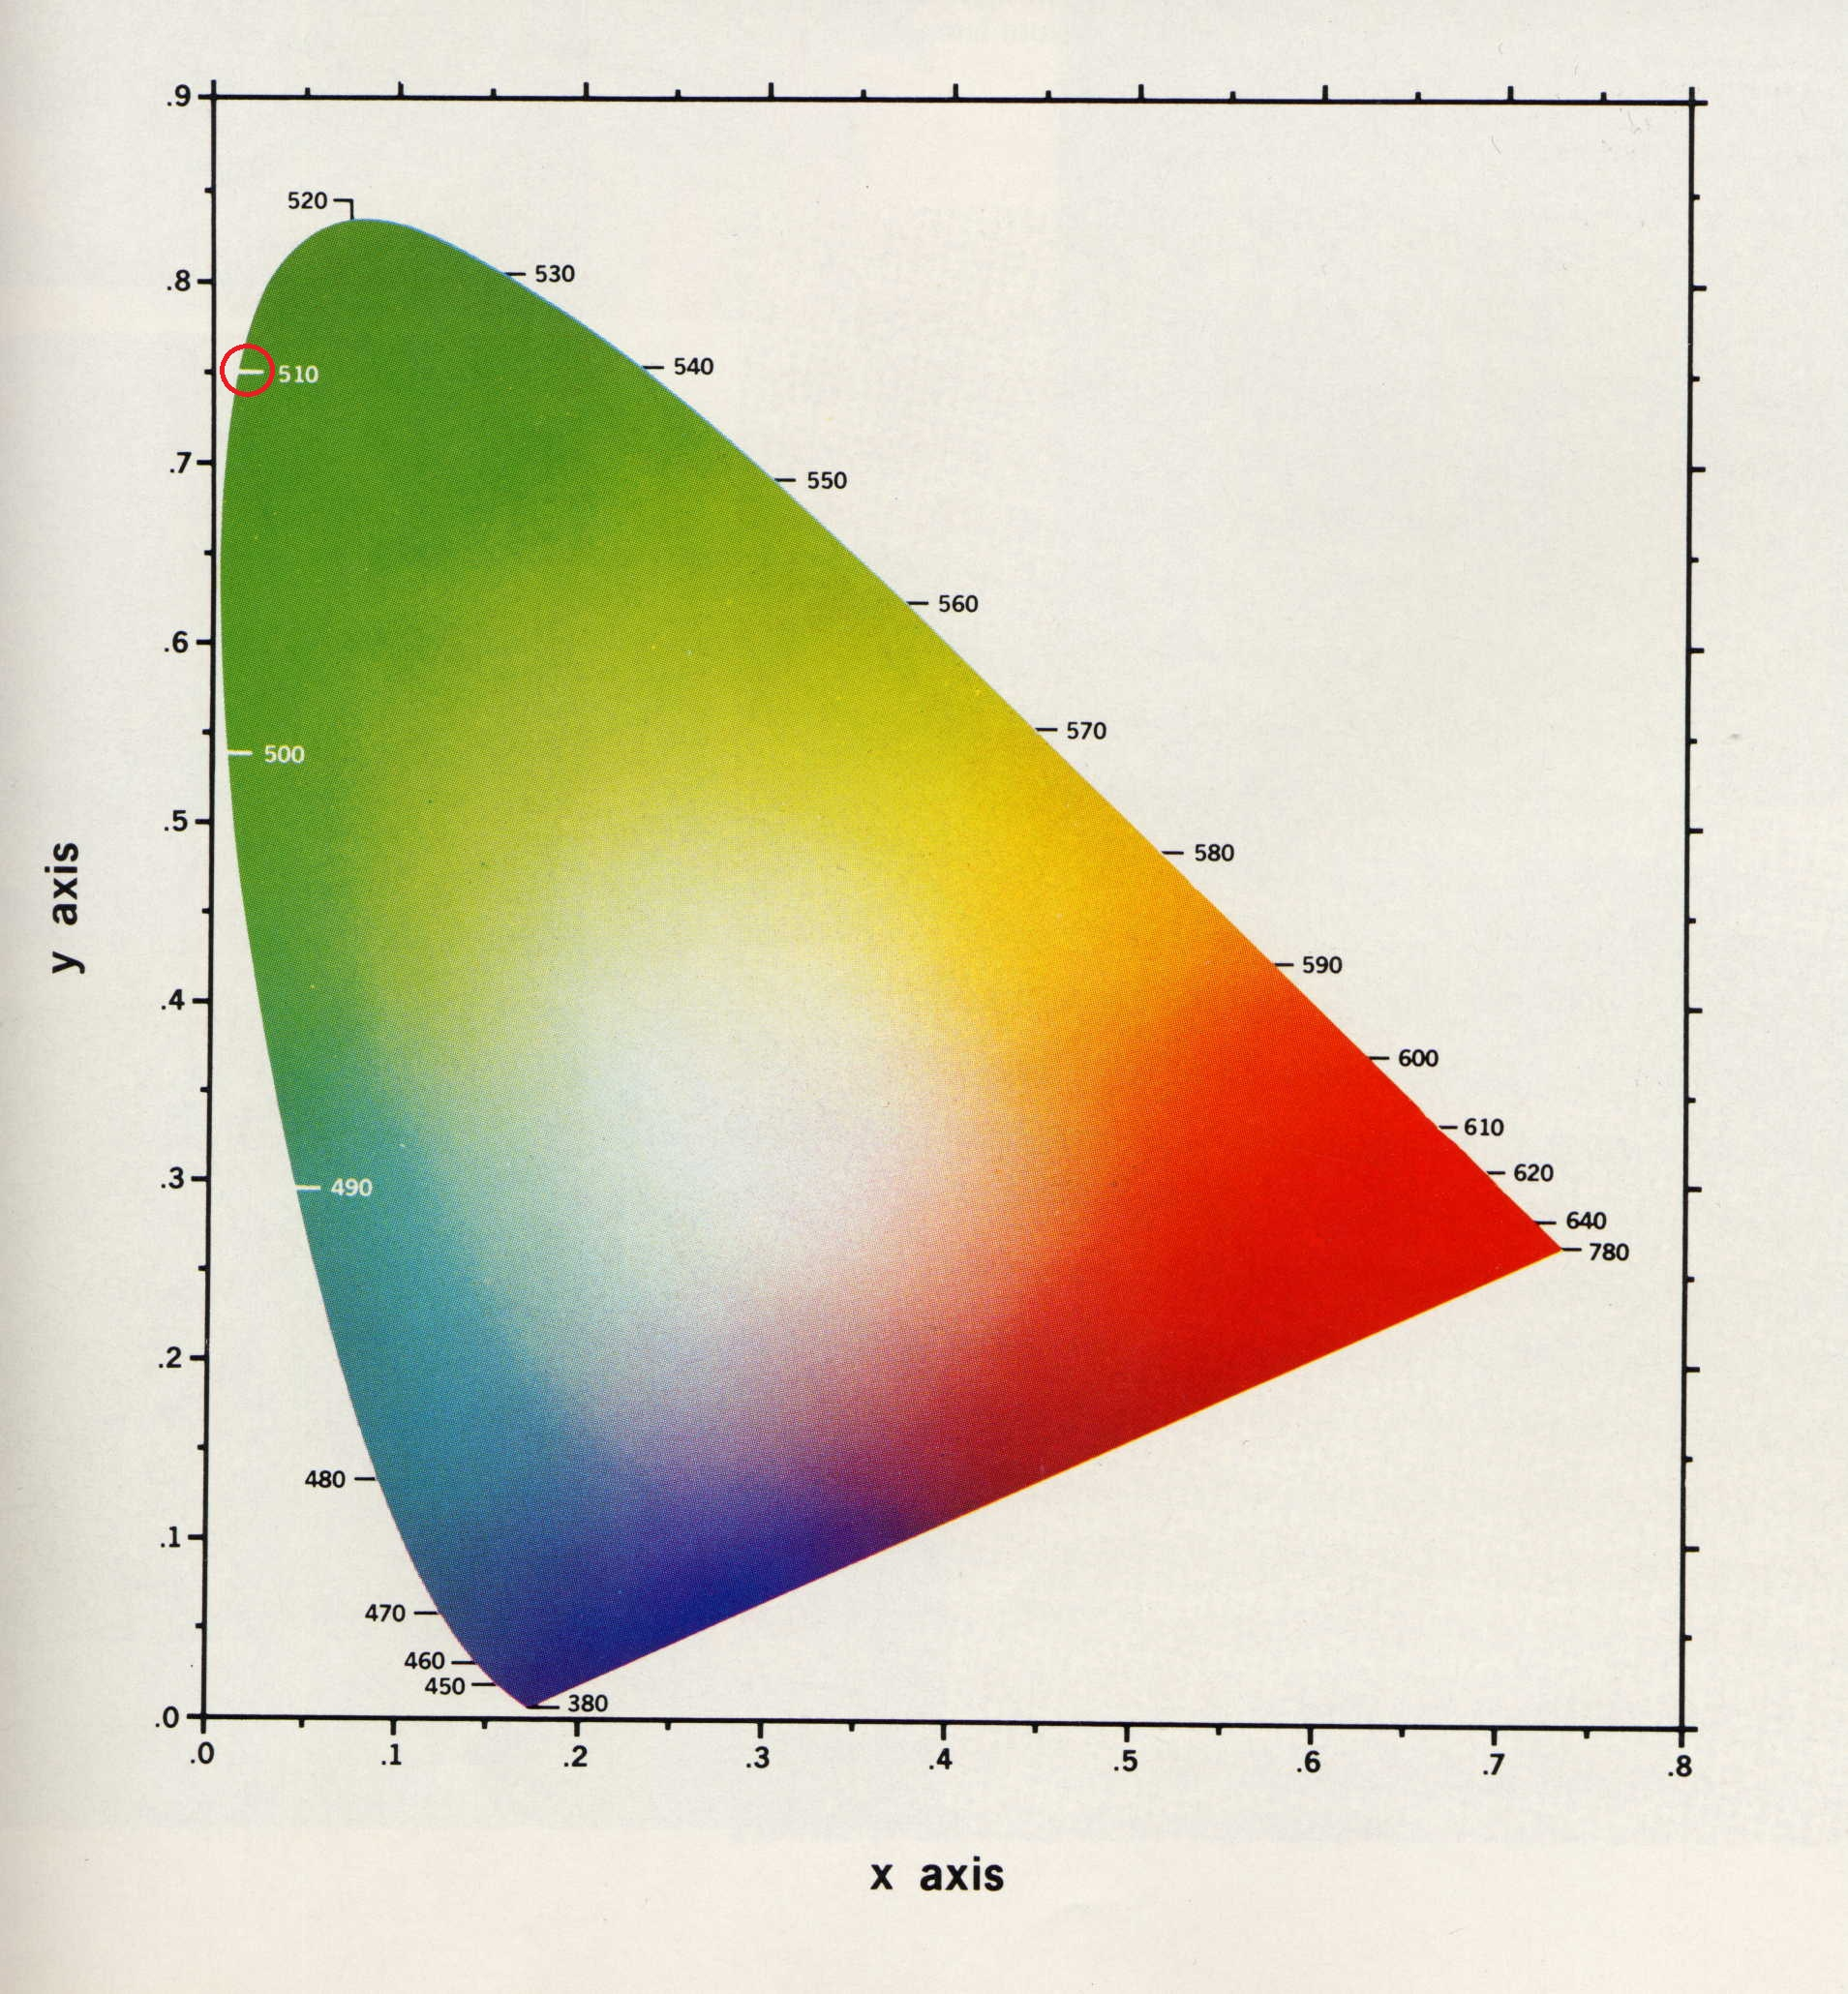
\includegraphics[width=0.4\textwidth]{2n.jpg}
\end{center}
o)Repeat process as described in n) DW = 610nm
\begin{center}
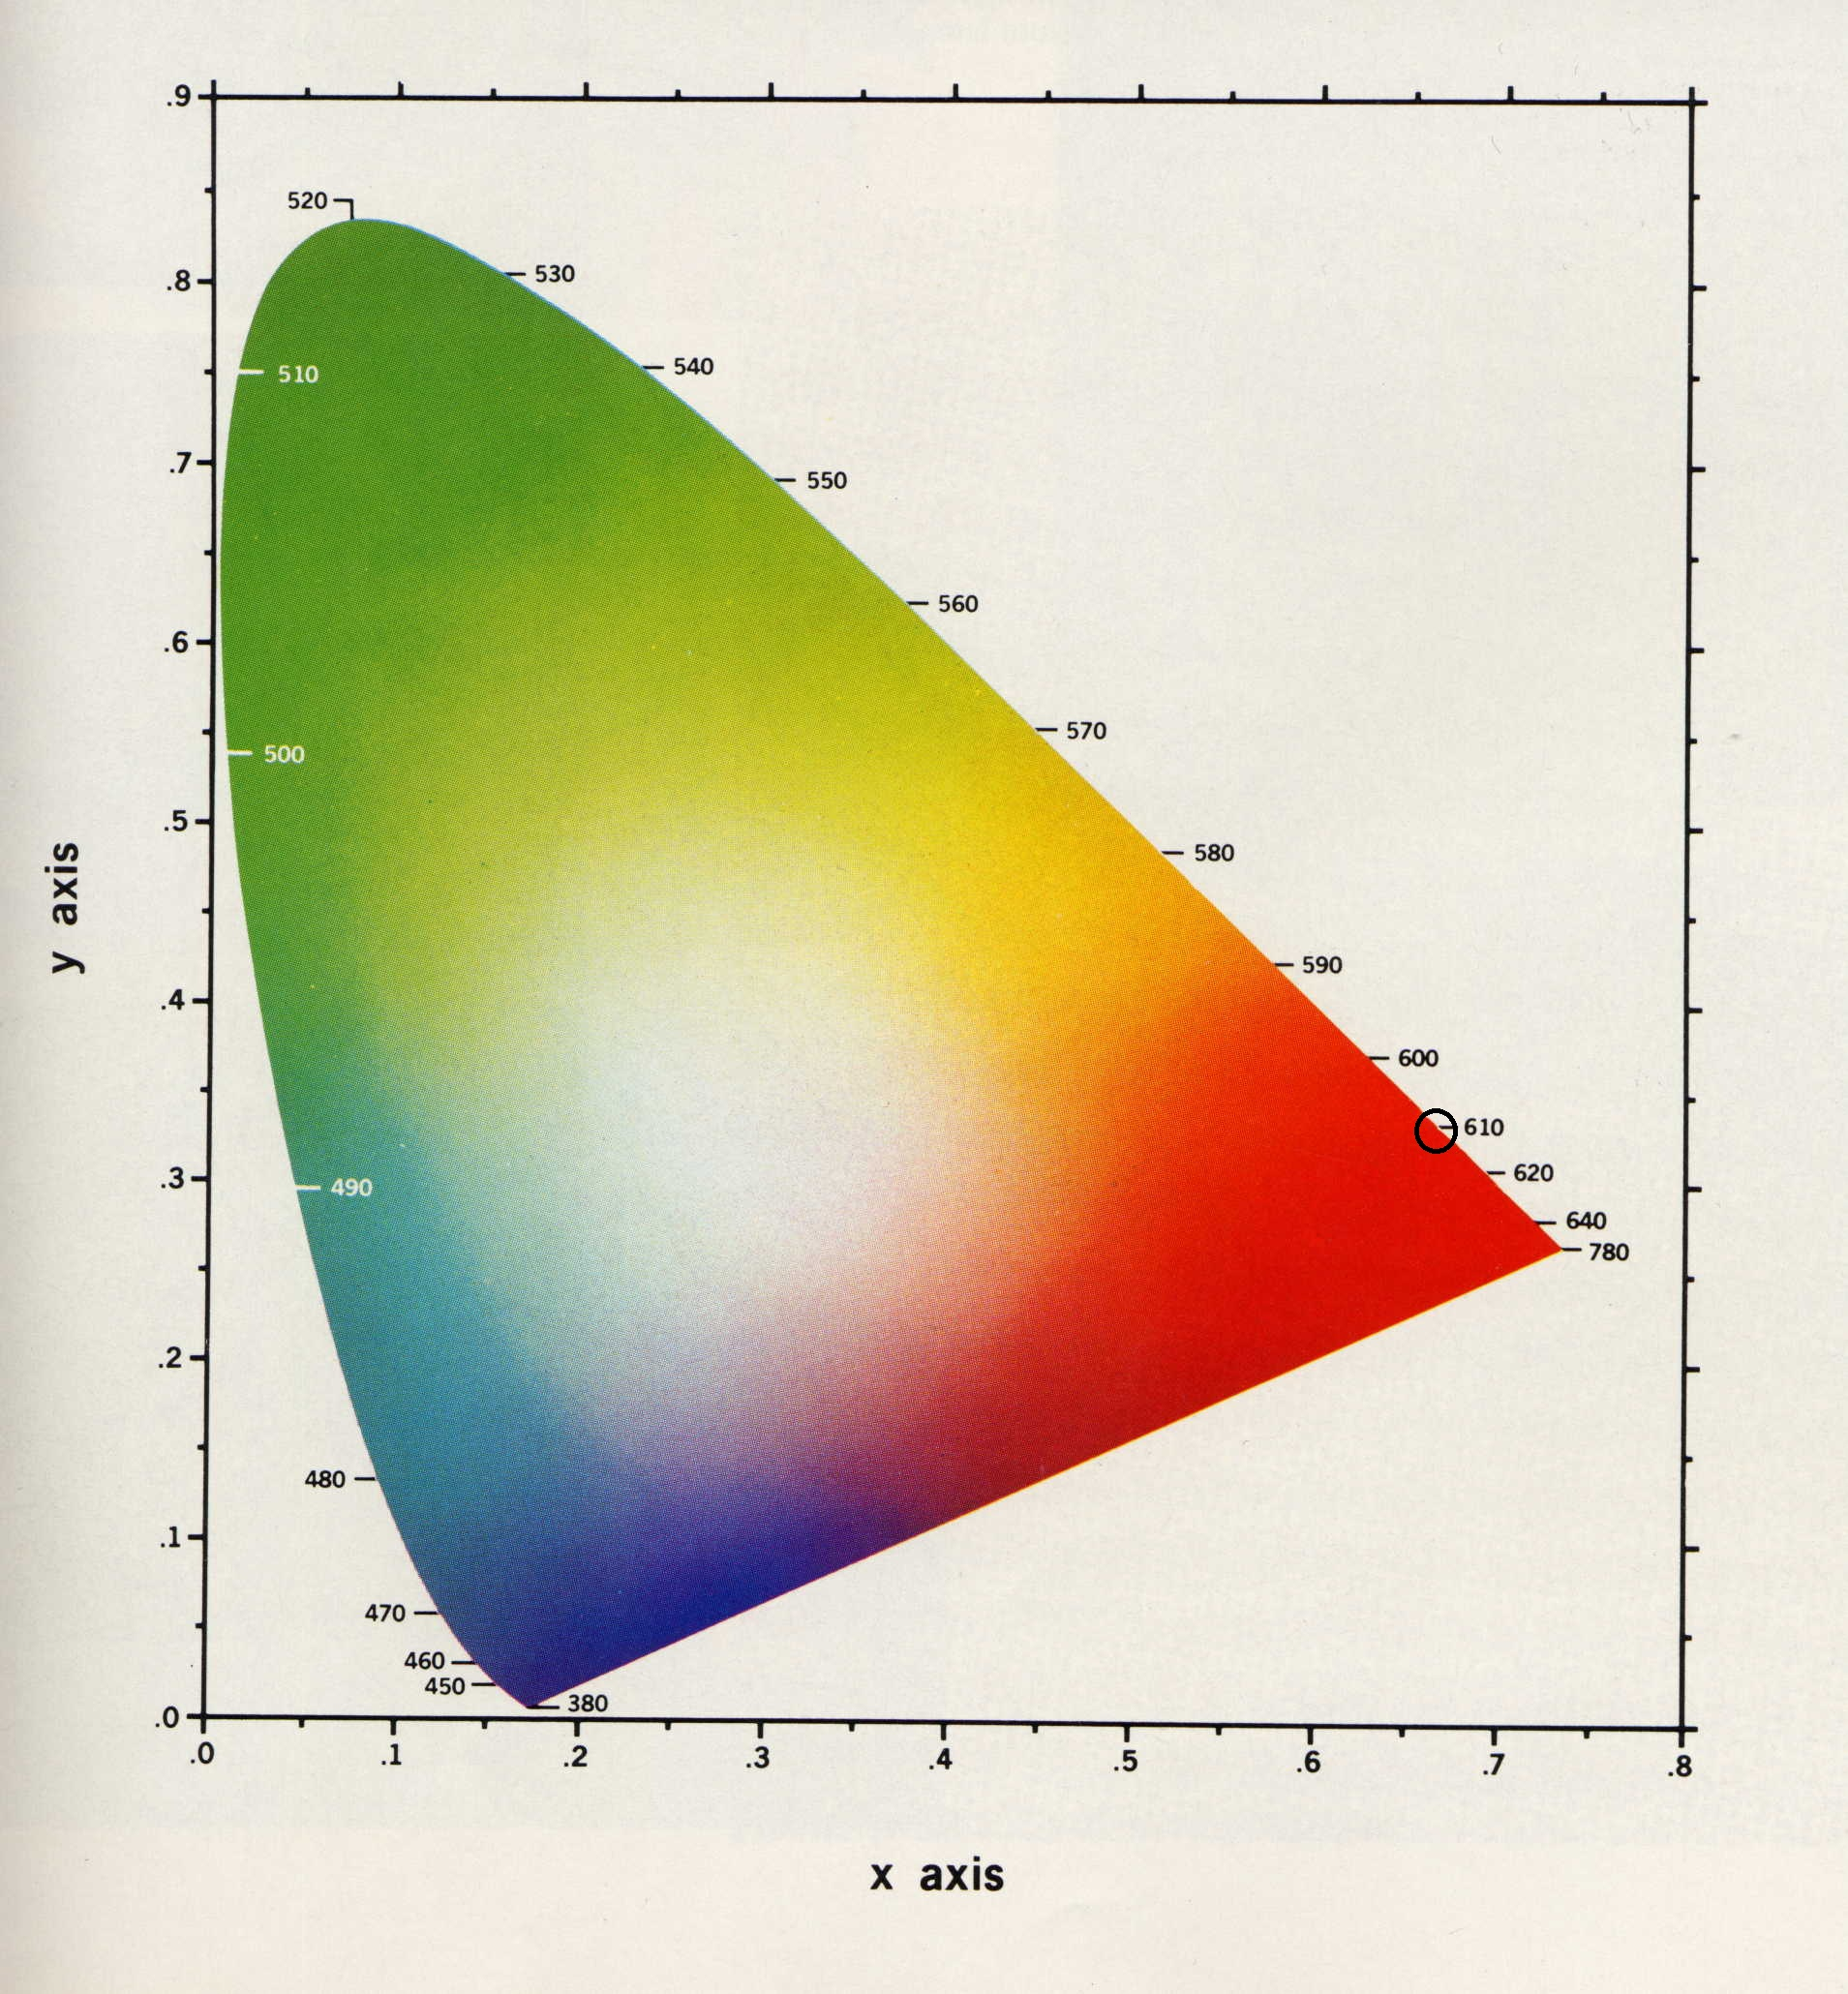
\includegraphics[width=0.4\textwidth]{2o.jpg}
\end{center}
p) DW = 520nm
\begin{center}
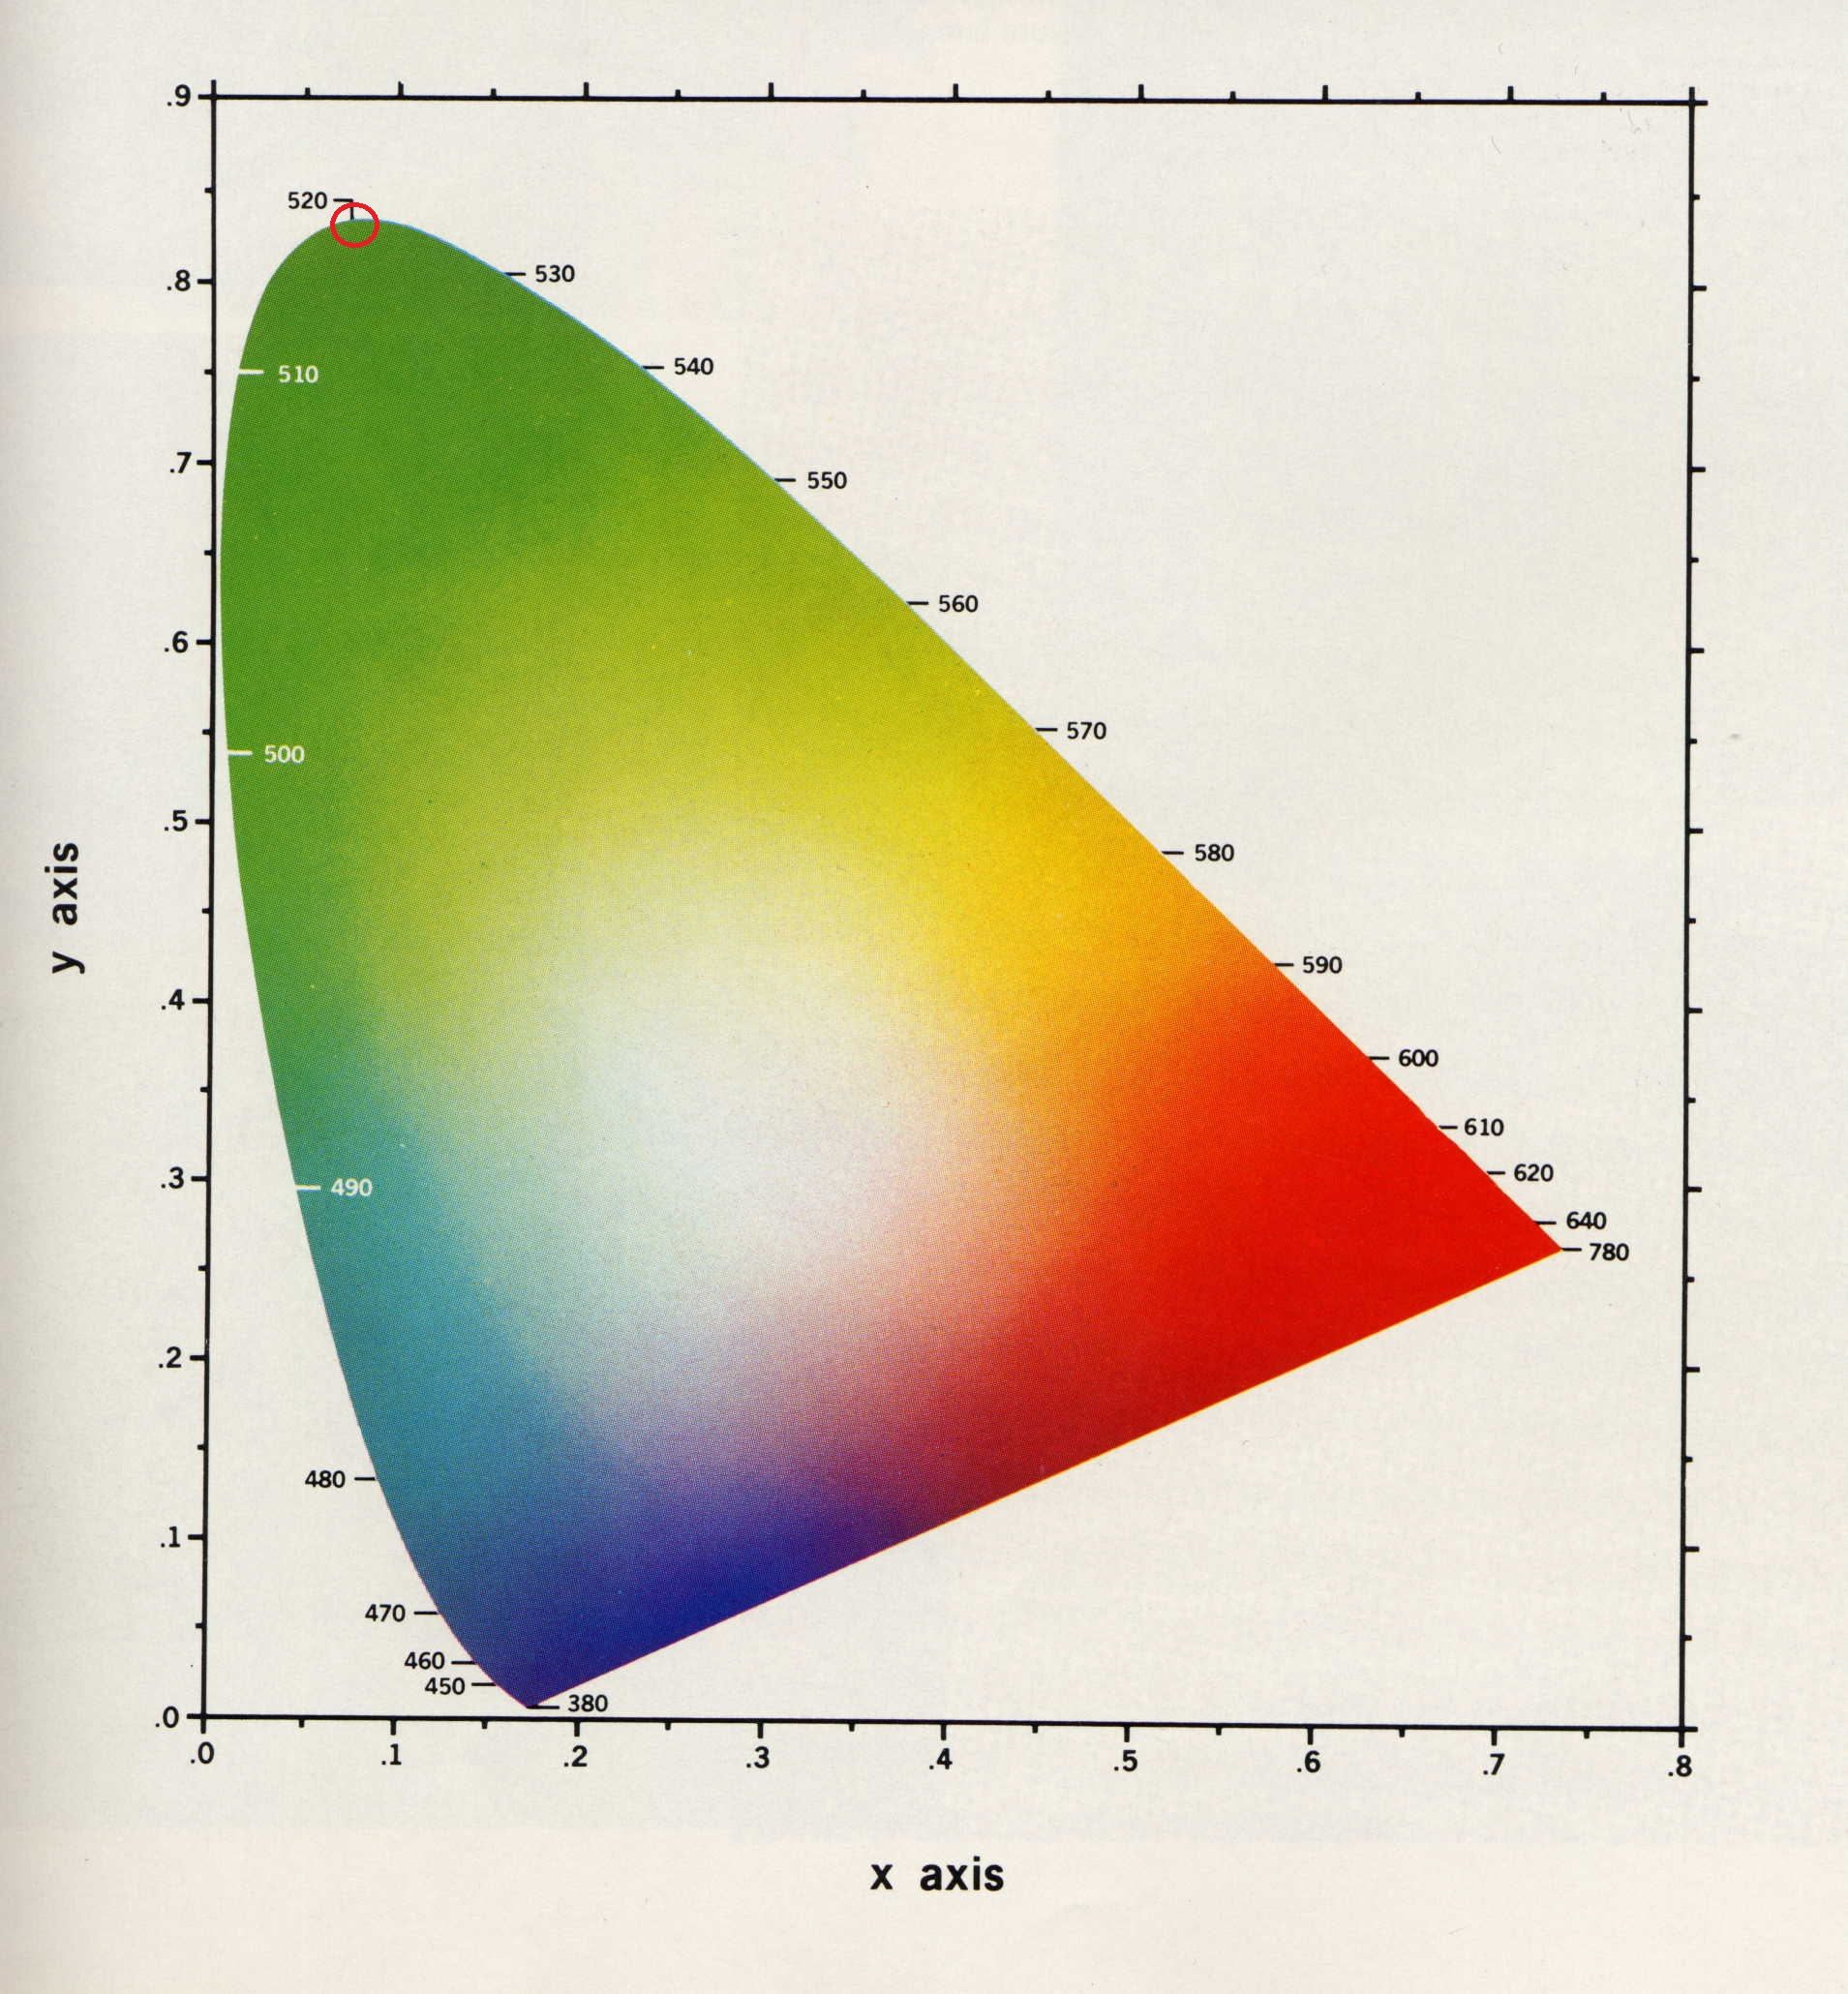
\includegraphics[width=0.4\textwidth]{2p.jpg}
\end{center}
q) ??????lolwut (human eye is more sensitive to green afaik)
\section{}
a) Look up figure 1.5
\begin{gather}  
R = I K_{R} cos\theta \\
G = I K_{G} cos\theta \\
B = I K_{B} cos\theta \\
cos\theta = \bar{n}\bar{l} \\
\text{If the surface is flat then }\ \theta = 0 \text{ and }\ cos\theta = 1 \text{ thus I is constant.}\ \\
\text{In the later case .. ?? to be updated}\
\end{gather}
b) R, G and B will change accordingly \\
c) \\
\begin{center}
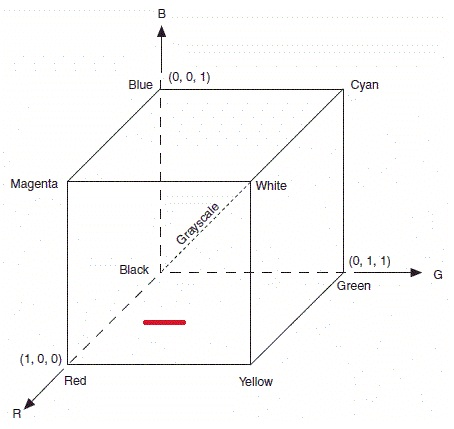
\includegraphics[width=0.4\textwidth]{rgbcube.jpg}
\end{center}
d)
\begin{gather}  
R = I K_{R} cos\theta \\
G = I K_{G} cos\theta \\
\frac{R}{G} = \frac{I K_{R} cos\theta }{I K_{G} cos\theta } = \frac{K_{R}}{K_{G}} \\
\text {independent of I; dependent only on the colors of the object}\
\end{gather}
e)\\
f)\\

\begin{gather}  
\text{Proof that }\ \frac{R}{G} \text{is color invariant to shiny surfaces}\ \\
\frac{R}{G} = \frac{I K_{R} cos\theta + I K_{S} cos^{n}\alpha}{I K_{G} cos\theta + I K_{S} cos^{n}\alpha} = 
\text {independent of I; dependent only on the colors of the object}\ \\
\text{Proof that}\ \frac{R-G}{R-B} \text{is color invariant to shiny surfaces}\ \\
\frac{R-G}{R-B} =  \frac{I K_{R} cos\theta + I K_{S} cos^{n}\alpha - (I K_{G} cos\theta + I K_{S} cos^{n}\alpha)}{I K_{R} cos\theta + I K_{S} cos^{n}\alpha - (I K_{B} cos\theta + I K_{S} cos^{n}\alpha } = \\
= \frac{I cos\theta(K_{R}-K_{G})}{I cos\theta(K_{R}-K_{B})} = \frac{K_{R}-K_{G}}{K_{R}-K_{B}} \\
\text{only dependent on the color of the object}\
\end{gather}
\end{document}
